\documentclass[11pt,a4paper]{report}

% ---------- Page geometry ----------
\usepackage[margin=2.7cm,headheight=14pt]{geometry}

% ---------- Fonts & typography ----------
\usepackage[utf8]{inputenc}
\usepackage[T1]{fontenc}
\usepackage{lmodern}
\usepackage{microtype}
\usepackage{parskip}
\usepackage{amsmath}

% ---------- Tables, figures, color ----------
\usepackage{graphicx}
\usepackage{booktabs}
\usepackage{array}
\usepackage{longtable}
\usepackage{float}
\usepackage{caption}
\usepackage{subcaption}
\usepackage{xcolor}
\usepackage{tcolorbox}
\tcbuselibrary{skins,breakable}
\usepackage{enumitem}
\usepackage{placeins}
\usepackage{multicol}

% ---------- Headers / footers ----------
\usepackage{fancyhdr}
\pagestyle{fancy}
\fancyhf{}
\fancyhead[L]{\small\itshape\leftmark}
\fancyhead[R]{\small\itshape Absence-seizure detection in EEG}
\fancyfoot[C]{\thepage}
\renewcommand{\headrulewidth}{0.4pt}
\renewcommand{\footrulewidth}{0pt}

\fancypagestyle{plain}{%
  \fancyhf{}
  \fancyfoot[C]{\thepage}
  \renewcommand{\headrulewidth}{0pt}
}

% ---------- Colors ----------
\definecolor{seizureteal}{HTML}{0B7285}
\definecolor{inkdark}{HTML}{0F172A}
\definecolor{panelgray}{HTML}{F5F7FA}
\definecolor{warnamber}{HTML}{B45309}

% ---------- Chapter/section styling ----------
\usepackage{titlesec}
\titleformat{\chapter}[hang]
  {\normalfont\huge\bfseries\color{inkdark}}{\thechapter}{20pt}{\Huge}
\titlespacing*{\chapter}{0pt}{0pt}{30pt}
\titleformat{\section}{\normalfont\Large\bfseries\color{seizureteal}}{\thesection}{10pt}{}
\titleformat{\subsection}{\normalfont\large\bfseries}{\thesubsection}{8pt}{}

% ---------- Hyperlinks (load last) ----------
\usepackage[hidelinks,colorlinks=true,linkcolor=seizureteal,citecolor=seizureteal,urlcolor=seizureteal]{hyperref}
\usepackage[capitalize]{cleveref}

% ---------- Graphics search path ----------
\graphicspath{{figures/}}

% ---------- Chapter-summary box ----------
\newtcolorbox{summarybox}{%
  enhanced, breakable, colback=panelgray, colframe=seizureteal,
  boxrule=0.6pt, arc=2pt, left=8pt, right=8pt, top=6pt, bottom=6pt,
  title={Chapter summary}, fonttitle=\bfseries\color{white},
  colbacktitle=seizureteal, coltitle=white
}

\newtcolorbox{pendingbox}{%
  enhanced, breakable, colback=yellow!8, colframe=warnamber,
  boxrule=0.6pt, arc=2pt, left=8pt, right=8pt, top=6pt, bottom=6pt,
  title={Pending / not yet finished}, fonttitle=\bfseries\color{white},
  colbacktitle=warnamber, coltitle=white
}

% ---------- Misc ----------
\setlength{\parindent}{0pt}
\setlength{\parskip}{6pt}
\renewcommand{\arraystretch}{1.15}

\title{\Huge\textbf{Detecting Absence Seizures in EEG}\\[6pt]
  \Large A classical machine-learning pipeline, built from the raw recordings up,\\
  measured against a deep-learning baseline}
\author{Wael Hammali\\\small École Nationale d'Ingénieurs de Tunis}
\date{\today}

\begin{document}

% ---------- Title page ----------
\begin{titlepage}
  \centering
  \vspace*{2cm}
  {\small\bfseries\color{seizureteal} DATA-MINING PROJECT\par}
  \vspace{0.3cm}
  \rule{0.4\linewidth}{0.8pt}\par
  \vspace{1.5cm}
  {\Huge\bfseries\color{inkdark} Detecting Absence Seizures\\[4pt] in EEG\par}
  \vspace{1cm}
  {\Large A classical machine-learning pipeline, built from the raw recordings\\
   up, and measured, honestly, against a deep-learning baseline.\par}
  \vfill
  \begin{minipage}{0.45\linewidth}
    \raggedright
    \textbf{Wael Hammali}\\
    École Nationale d'Ingénieurs de Tunis
  \end{minipage}
  \hfill
  \begin{minipage}{0.45\linewidth}
    \raggedleft
    21 recordings \textbullet{} 19 EEG channels\\
    93 confirmed seizures
  \end{minipage}
  \vspace{1.5cm}
  \par{\large \today\par}
\end{titlepage}

\pagenumbering{roman}
\tableofcontents
\listoffigures
\listoftables
\clearpage
\pagenumbering{arabic}

\chapter{Introduction}
\label{chap:introduction}

An absence seizure is short. It lasts only a few seconds, it shows up across the whole scalp
at once rather than in one spot, and on a long EEG recording it is genuinely easy for a human
reader to miss. Clinically, it is described as a generalized, roughly 3~Hz spike-and-wave
discharge, usually lasting 3 to 20 seconds, and it is seen mostly in children. Catching every
one of these events by eye, in hours of recording, is tedious and error-prone work.

This project builds an automatic detector for absence seizures, trained and evaluated on 21
real clinical EEG recordings. The goal was never simply to produce a high score on a benchmark;
it was to build something a clinician could actually trust: a detector that says, for a given
recording, here is where I believe a seizure happened, and here is how often I am wrong. That
second half --- being honest about false alarms, not just about seizures found --- shaped
almost every decision in this project, from how the data was split to how a detection is
scored.

\section{Objectives}

Three things were set out from the start:

\begin{enumerate}[leftmargin=1.4em]
  \item \textbf{Build a reliable classical pipeline.} Take the raw EEG recordings, clean and
    align them against their seizure annotations, filter and window the signal, extract
    hand-crafted features, and train a set of classical machine-learning models to detect
    seizures event by event, not just window by window.
  \item \textbf{Push past the obvious baseline.} Once a working pipeline exists, try to improve
    it: rebalancing the training data, augmenting the rare seizure class, and blending several
    models together, and report honestly which of these actually helped.
  \item \textbf{Compare against deep learning.} Train a convolutional neural network directly on
    the raw filtered signal, with no hand-crafted features at all, and measure it against the
    classical pipeline under the same evaluation rules, to see whether a model that learns its
    own representation can do better than one built on 320 hand-designed numbers per window.
  \item \textbf{Make the results usable.} Package everything behind a web application so that
    the recordings, the model predictions, and the comparison between models can actually be
    explored, not just read off a table in a report.
\end{enumerate}

\section{What this report covers}

The chapters that follow tell this story in the order it actually happened. \Cref{chap:rawdata}
covers the raw data itself: 22 recordings that started as raw MATLAB files with no declared
sampling rate, no declared amplitude unit, and seizure times stored as clock times with no
absolute start time to anchor them to --- and the concrete decisions made to turn that into a
clean, trustworthy 21-recording, 93-seizure dataset. \Cref{chap:preprocessing} covers the signal
processing and feature extraction built on top of that clean data.
\Cref{chap:classicalml,chap:augmentation,chap:ensemble} cover the classical machine-learning
pipeline: twelve models, three training strategies, and what helped and what did not.
\Cref{chap:deeplearning} covers the deep-learning comparison, including a real bug that produced
a real crash and how it was found and fixed. \Cref{chap:evaluation} pulls the evaluation
methodology together across all of the above, since several different threshold-selection
protocols are used in this project and keeping them straight matters for a fair comparison.
\Cref{chap:application} describes the web application built to explore the results.
\Cref{chap:lessons} is an honest account of what went wrong along the way, and
\Cref{chap:conclusion} closes with what the project actually achieved and what is still left to
do.

\begin{summarybox}
This project detects absence seizures in EEG, event by event, starting from 22 raw clinical
recordings with no declared sampling rate or amplitude unit and an annotation workbook that
needed real detective work to align. The result is a classical machine-learning pipeline (12
models), a deep-learning comparison, and a web application to explore both --- reported here
with every number traced back to its source, and every negative result kept in, not hidden.
\end{summarybox}

\chapter{The Raw Data}
\label{chap:rawdata}

Before any model could be trained, the raw data had to be understood, cleaned, and in several
places, repaired by hand. This chapter describes what the recordings actually looked like on
arrival, what was missing from them, and the concrete decisions taken to turn 22 raw recordings
and one imperfect annotation workbook into the 21-recording, 93-seizure dataset that everything
else in this report is built on.

\section{What we actually started with}

The project began with 22 recordings. Each one is a pair of raw MATLAB files --- one holding the
signal, one holding a header of technician notes --- plus a single \texttt{Annotations.xlsx}
workbook shared across all 22, listing each patient's seizure times and free-text notes.

Every recording was sampled at 256~Hz. This was not written anywhere in a header field: it had
to be decoded from the structure of the raw sample blocks themselves, which are organized in
1-second chunks of exactly 256 samples each.

The full channel montage, where present, was 19 EEG channels in the standard 10--20 layout, plus
an SLI channel (a pulse marker used during light stimulation testing), an ECG channel, and, in
some recordings, two EMG channels. Channel order was \emph{not} consistent from one file to the
next, so every channel was matched by its name, never trusted to sit in the same column twice.

Three things that should have been documented were not, and each had to be recovered from the
data itself rather than assumed:

\begin{itemize}[leftmargin=1.4em]
  \item \textbf{Sampling rate.} Not in any header field; decoded from the 256-sample blocks.
  \item \textbf{Channel order.} Not consistent file to file; channels are matched by name only.
  \item \textbf{Amplitude units.} No \texttt{varUnits} field, no description field, on any
    signal. Amplitude is reported throughout this project as ``unit not confirmed,'' and is
    never labeled microvolts without proof.
\end{itemize}

\section{What we cut, and why}

\subsection{One recording dropped entirely}

Recording \texttt{200625A\_F} had two problems at once: it carried only 8 of the 19 EEG
channels --- the 8 that happen to be common to every one of the 22 recordings --- and it had
zero seizure annotations of any kind.

Missing annotations do not prove a recording is seizure-free; they could just as easily mean a
label was never entered. Labeling this recording as a seizure-free control, on no evidence
either way, would have fed the model a guess dressed up as a fact. It was dropped entirely
instead. This leaves 21 recordings, every one of them with the full 19-channel EEG montage ---
the number quoted everywhere else in this report.

\subsection{What feeds the model, and what never does}

Only the 19 EEG channels are ever used as model input. The other signals and fields collected
alongside them are kept, but strictly as an audit tool, applied only \emph{after} a model has
already made its decisions:

\begin{itemize}[leftmargin=1.4em]
  \item \textbf{SLI pulses} --- checked against false alarms, to see whether a false alarm lands
    on a stimulation pulse.
  \item \textbf{ECG and EMG} --- checked for muscle-artifact bursts (an EMG RMS spike) behind a
    false alarm.
  \item \textbf{HPN notes} (the technician's hyperpnea markers, a seizure-provocation technique)
    --- checked for false alarms that coincide with a provocation period.
  \item \textbf{Sex, age, seizure count, seizure type, and the undocumented
    \texttt{Intercrit} markers} --- kept as separate patient metadata, never mixed into the
    training table.
\end{itemize}

The distinction is deliberate: these extra channels and fields make a model's errors
explainable after the fact, without ever being allowed to quietly influence the decision itself.

\subsection{Two clocks that never agreed}

The signal and the annotation workbook each start their own internal clock at zero, but the raw
files never recorded an absolute wall-clock start time. Seizure times in the workbook, meanwhile,
are stored as clock times of day --- for example \texttt{10:35:06} --- not as seconds already
relative to the start of the recording.

The correct conversion is
\[
  \text{elapsed seconds} = \text{clock time of the annotation} - \text{recording start time},
\]
with a midnight rollover applied when a seizure's clock time wraps past 00:00. Two shortcuts
were considered and explicitly rejected: treating the workbook's time as if it were already
relative seconds, and anchoring everything on the time of the first seizure. Either one would
have quietly fabricated labels rather than recovered real ones.

\begin{figure}[H]
  \centering
  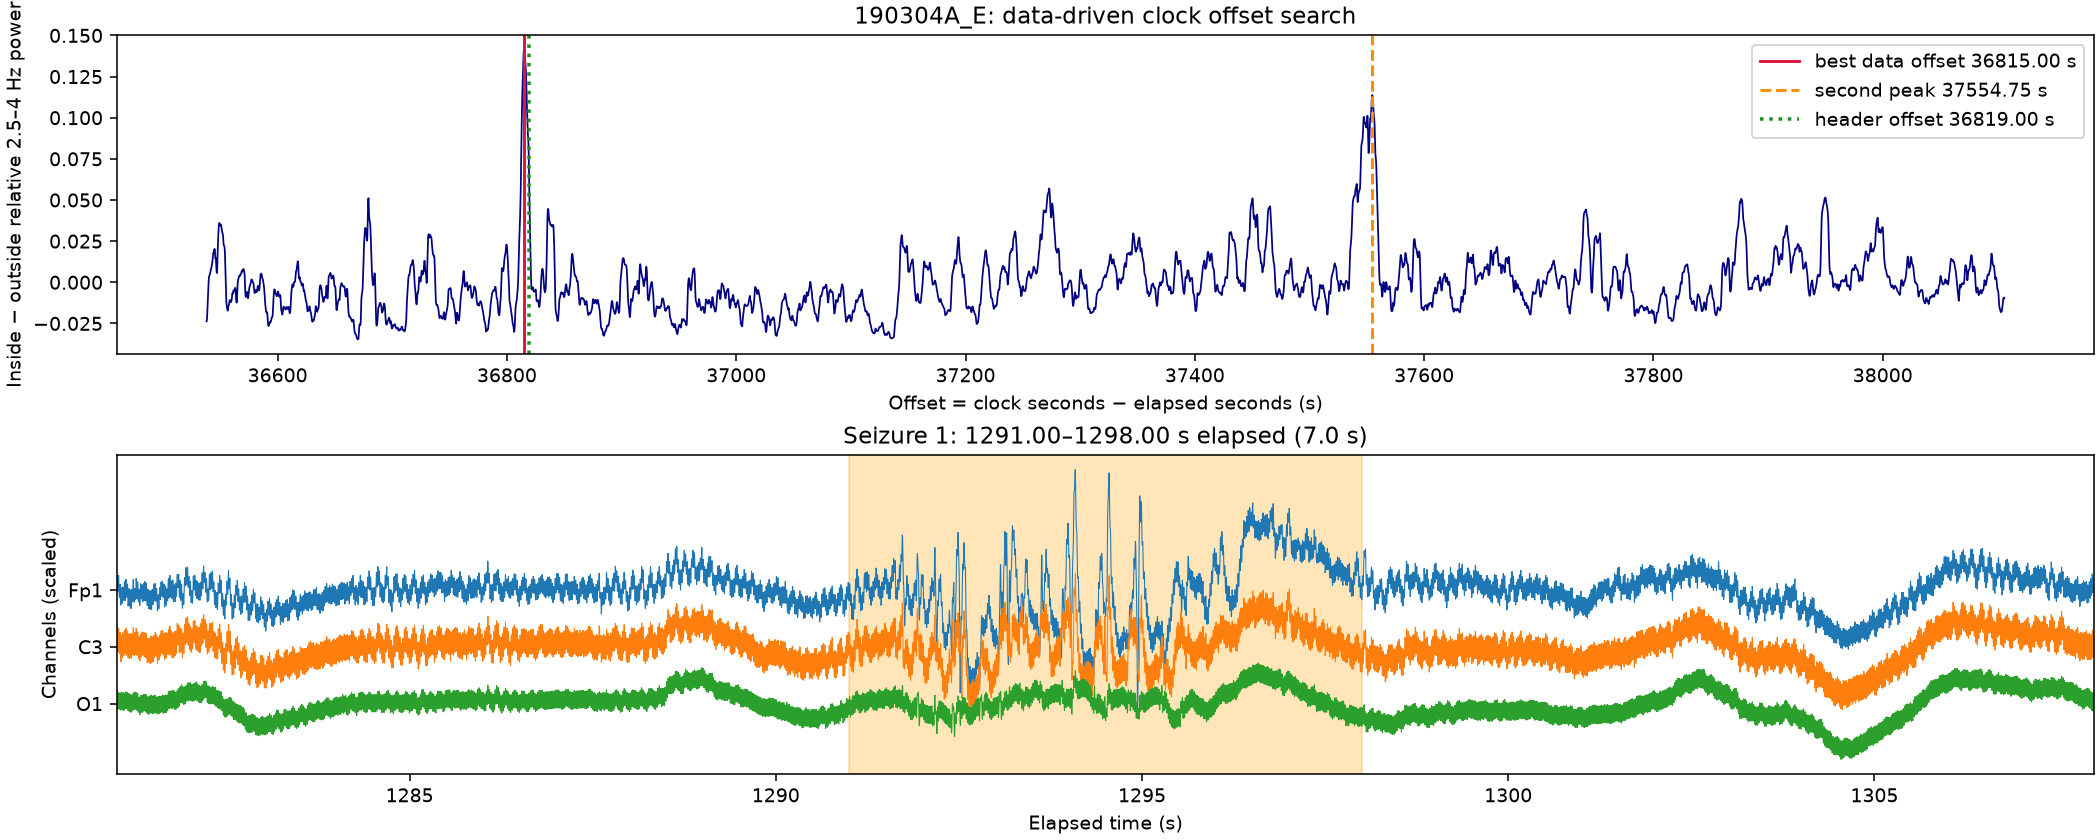
\includegraphics[width=0.85\linewidth]{offset_alignment/190304A_E_offset_alignment.png}
  \caption{Recovering the clock offset for recording \texttt{190304A\_E}: the technician's
    header markers are matched against the EEG signal itself to find the offset between the
    workbook's clock and the recording's internal clock.}
  \label{fig:offset-alignment-example}
\end{figure}

\subsection{When the labels disagreed, the signal decided}

Two recordings carried two conflicting candidate annotation rows each, with different proposed
seizure times for the same recording. Rather than pick a version by hand, each candidate
interval was scored against the real EEG: a seizure-likelihood score was computed inside the
candidate interval and outside it, and the candidate with the cleaner inside/outside separation
was kept.

\begin{table}[H]
  \centering
  \caption{Resolving the two conflicting annotation rows for \texttt{230406B\_A} by scoring each
    candidate against the real signal.}
  \label{tab:duplicate-rows}
  \begin{tabular}{lrrl}
    \toprule
    Candidate & Score & Inside/outside ratio & Decision \\
    \midrule
    Row 11 & 0.189 & 2.18 & Kept \\
    Row 19 & 0.173 & 2.09 & Dropped \\
    \bottomrule
  \end{tabular}
\end{table}

Recording \texttt{230515B\_G} was resolved the same way (row with ratio 4.08 kept over the row
with ratio 4.00). \texttt{210504B\_C}'s first seizure interval had a proposed end-time
correction that was validated the same way (score 0.306, ratio 2.61) and retained, and
\texttt{210427B\_C}'s official start time was validated likewise (score 0.306, ratio 2.70) and
included --- an important correction, since an earlier, now-archived version of the pipeline had
once excluded this recording for ``ambiguous alignment'' under a different, provisional
annotation set. That exclusion does not apply to the official dataset used in this report.

\begin{figure}[H]
  \centering
  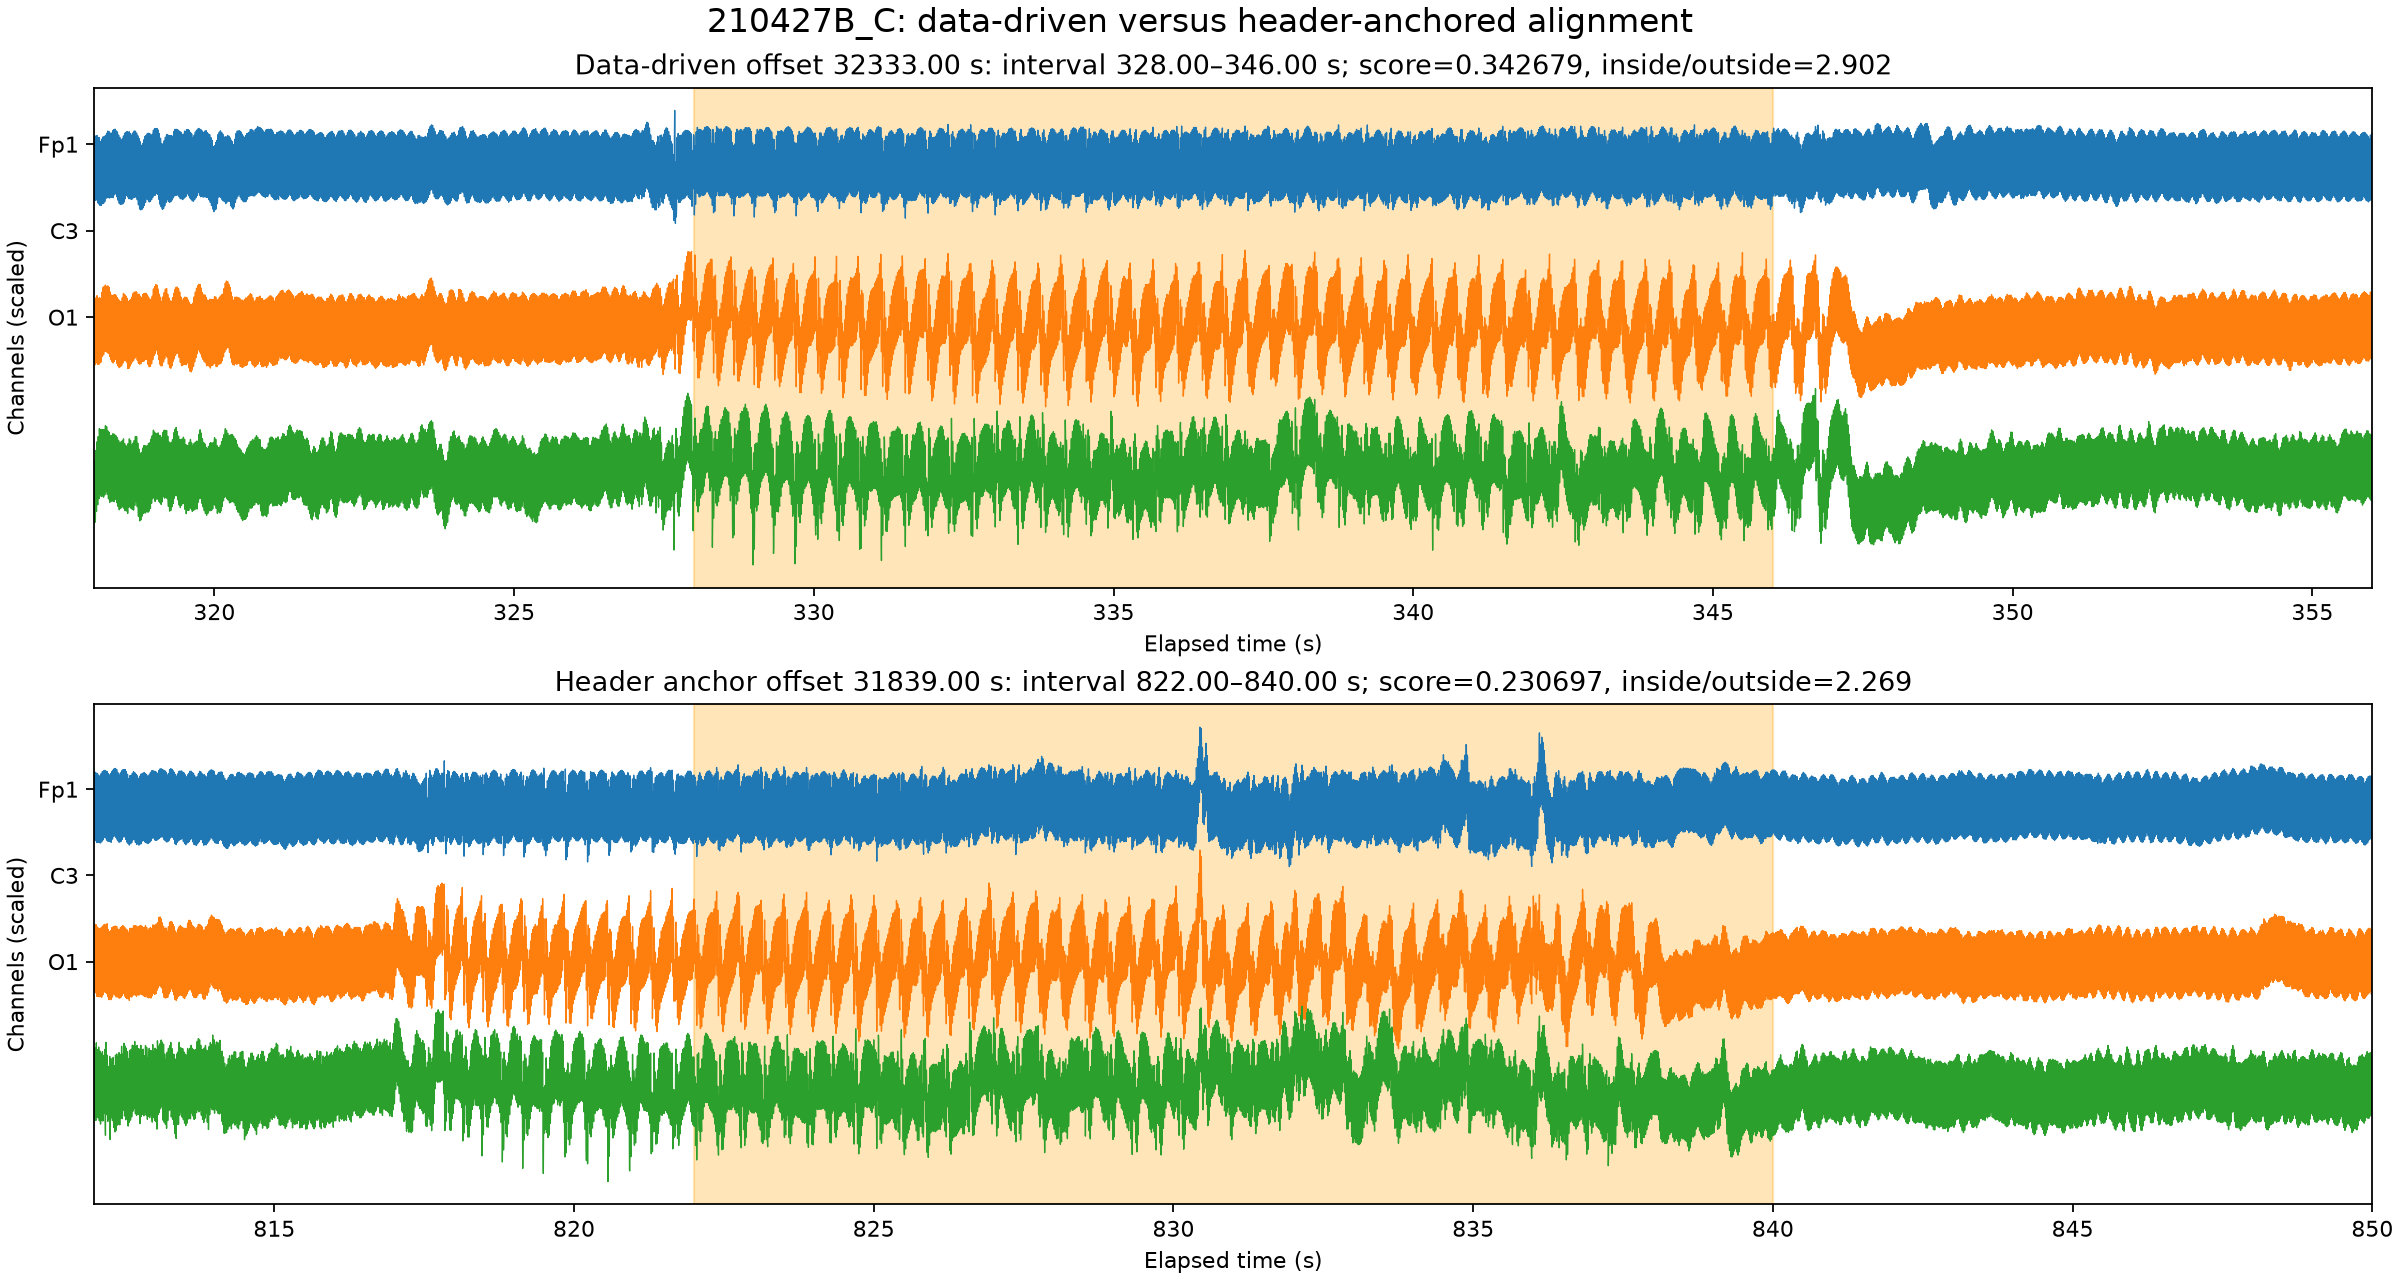
\includegraphics[width=0.85\linewidth]{offset_alignment/210427B_C_candidate_comparison.png}
  \caption{Comparing candidate seizure intervals for \texttt{210427B\_C} against the real
    signal, the method used to resolve every ambiguous or duplicate annotation row.}
  \label{fig:candidate-comparison}
\end{figure}

Two further recordings, \texttt{210204B\_C} and \texttt{210208B\_G}, are missing from the final,
corrected annotation workbook entirely. Both fall back to an earlier, provisional set of
intervals, rather than being invented or silently dropped.

\section{What survived the cleanup}

\begin{table}[H]
  \centering
  \caption{The dataset used throughout the rest of this report.}
  \label{tab:final-dataset}
  \begin{tabular}{lr}
    \toprule
    Recordings & 21 \\
    EEG channels per recording & 19 \\
    Confirmed, usable seizures & 93 \\
    Total recorded time & 8.73 hours (\texttt{models/registry.json}) \\
    \bottomrule
  \end{tabular}
\end{table}

From 22 recordings and one shared, imperfect workbook, this is the ground truth that every
later chapter is built on: the filter, the features, the twelve classical models, the deep
learning comparison, and the application all trace back to exactly these 21 recordings and
these 93 seizures.

\begin{summarybox}
The raw data arrived as 22 MATLAB recordings with no declared sampling rate, no declared
amplitude unit, inconsistent channel ordering, and seizure times with no absolute clock to
anchor them to. One recording was excluded for lacking both a full channel set and any
annotation; two recordings had genuinely conflicting annotation rows, resolved by scoring each
candidate against the real signal rather than by guessing; two more recordings, missing from the
final workbook, fell back to provisional intervals rather than being invented. The result is 21
recordings, 19 EEG channels each, 93 confirmed seizures --- the numbers used everywhere else in
this report.
\end{summarybox}

\chapter{Preprocessing}
\label{chap:preprocessing}

With a clean set of 21 recordings and 93 aligned seizures in hand, the next step was to turn
continuous EEG into something a classical machine-learning model can actually consume: short,
fixed-length windows, each described by a fixed set of numbers. This chapter covers the filter,
the windowing, and the feature extraction, in that order --- and explains why each choice was
made, not just what it was.

\section{The frequency filter}

Every recording is passed through a 4th-order Butterworth band-pass filter, 0.5--40~Hz, applied
\emph{zero-phase} --- forward and then backward through the signal, not a single forward pass.

Three separate decisions sit inside that one filter, each for its own reason.

\begin{itemize}[leftmargin=1.4em]
  \item \textbf{0.5~Hz low cutoff.} Strips slow baseline drift --- sweat, skin-potential drift,
    slow head movement --- without touching the frequency range where seizure activity and
    normal brain rhythms actually live.
  \item \textbf{40~Hz high cutoff.} Removes high-frequency muscle and movement noise, and sits
    safely below 50~Hz mains hum (the local electrical mains frequency), so that hum is
    attenuated along with everything else above 40~Hz.
  \item \textbf{Zero-phase filtering.} A normal, single-pass (causal) filter introduces a time
    lag. Filtering forward and backward cancels that lag out, so a filtered seizure's boundaries
    land on exactly the same timestamps as the original annotated boundaries. This matters
    because the entire evaluation later in this report depends on precise event timing.
\end{itemize}

\begin{figure}[H]
  \centering
  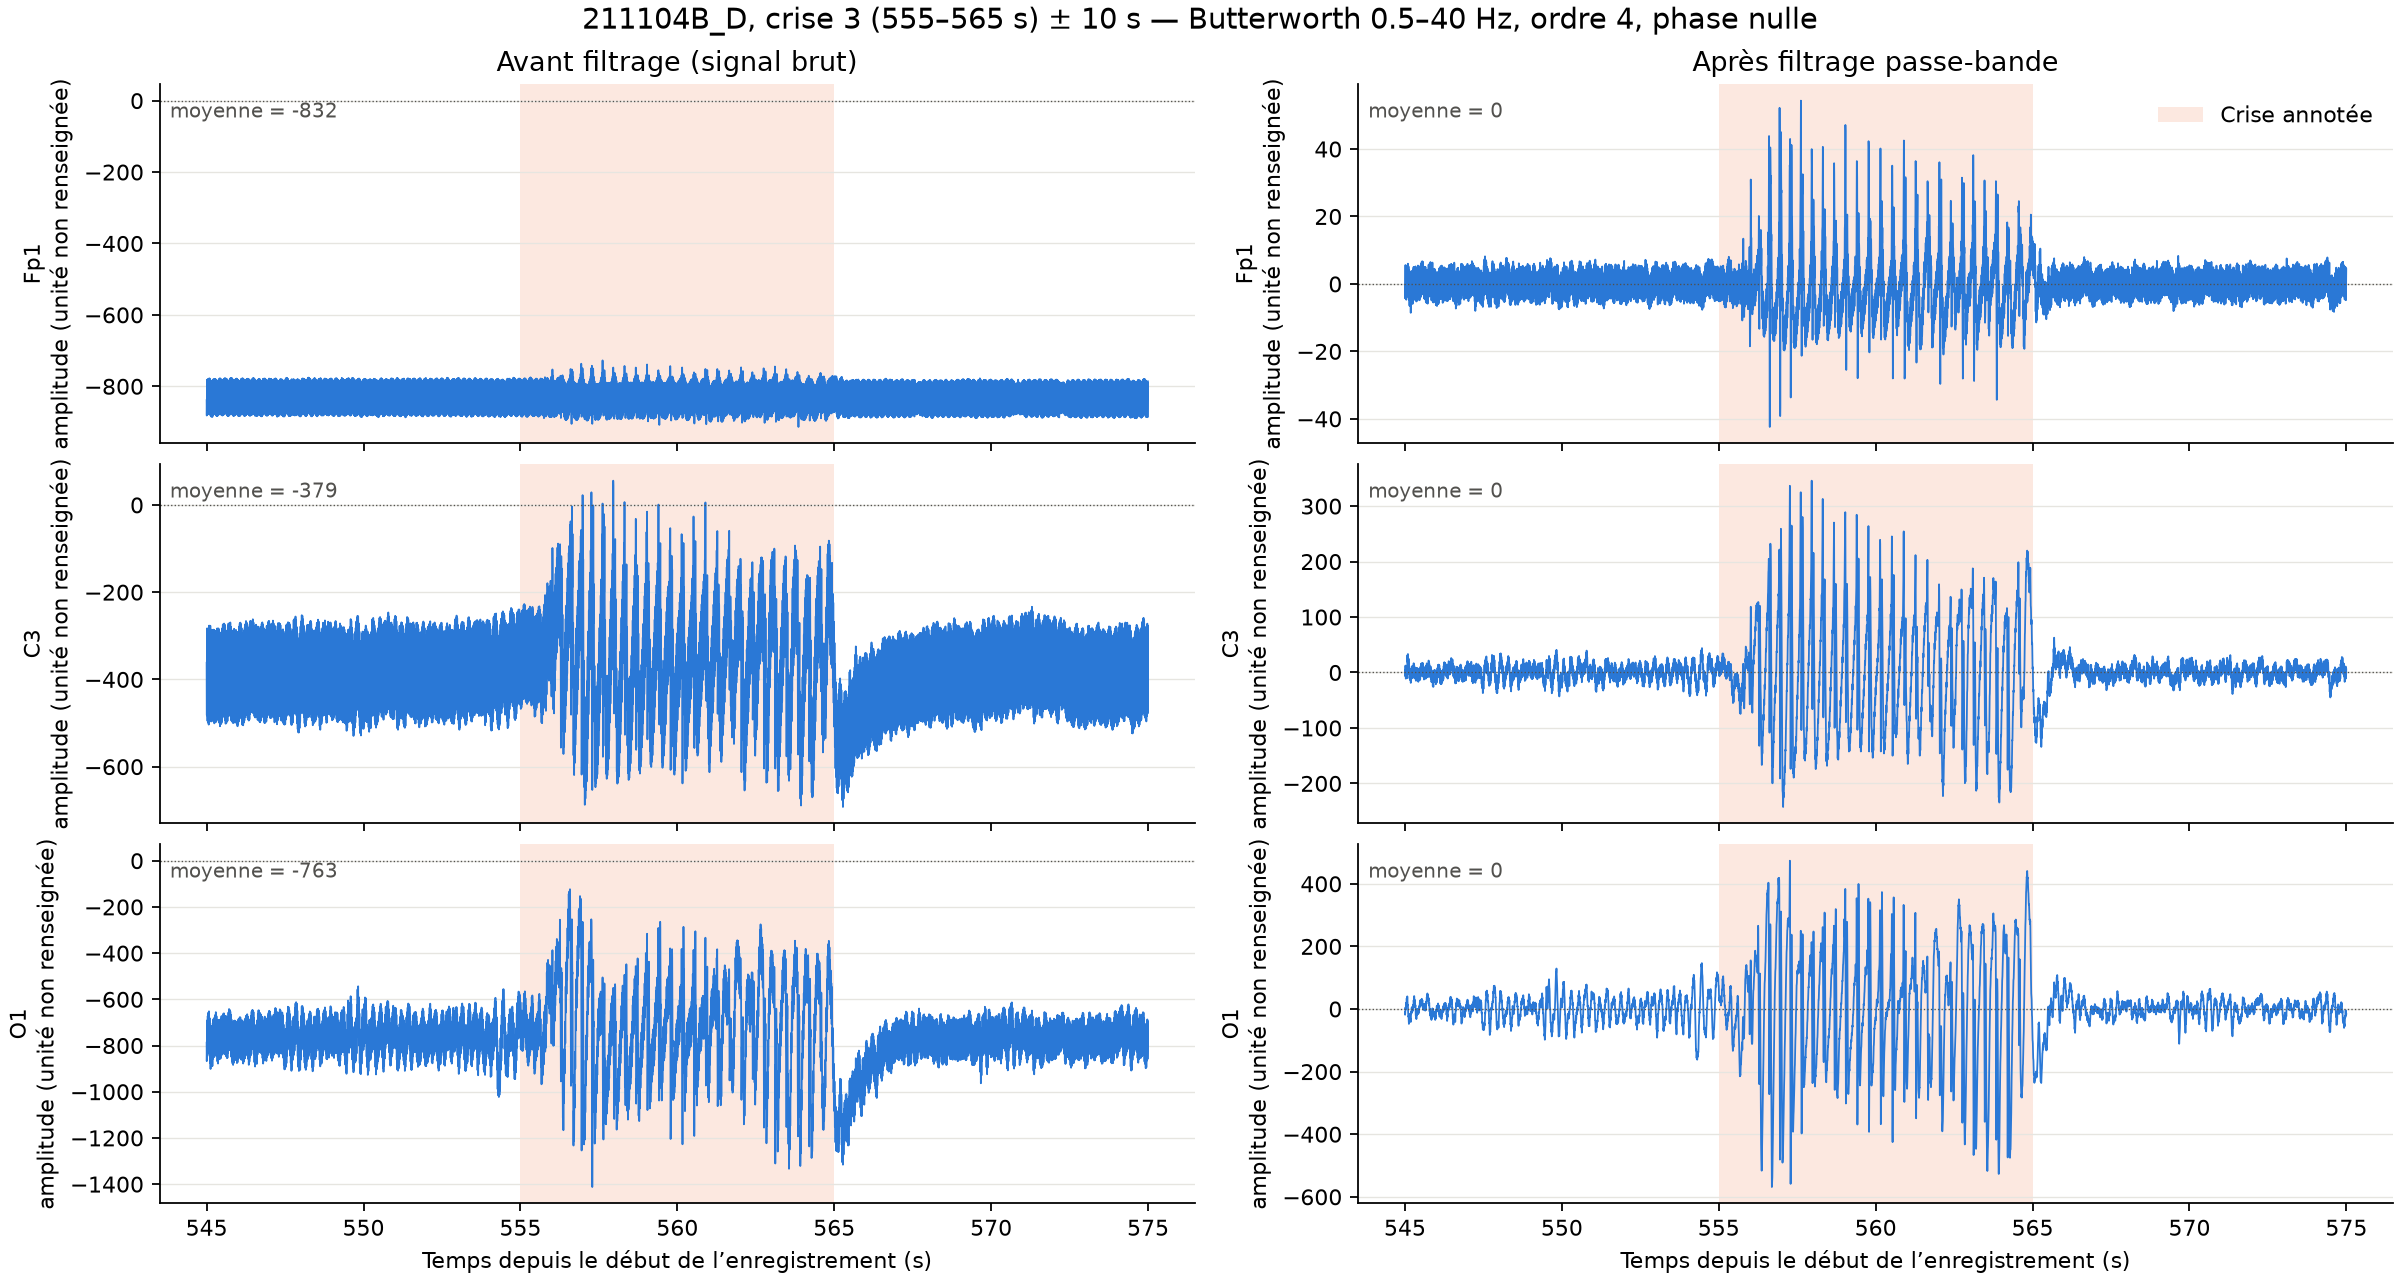
\includegraphics[width=0.9\linewidth]{official/preprocessing/211104B_D_seizure3_filtering.png}
  \caption{A real seizure segment from \texttt{211104B\_D} before and after the 0.5--40~Hz
    zero-phase band-pass filter.}
  \label{fig:filtering-example}
\end{figure}

\section{Windowing}

The filtered signal is cut into 2-second windows with 50\% overlap between consecutive windows.
A window is labeled as a seizure window (class 1) if at least half of its samples fall inside an
annotated seizure; otherwise it is labeled class 0.

This produces 31{,}419 windows in total: 1{,}244 of them seizure windows (3.96\%), and
30{,}175 non-seizure (96.04\%). Fewer than four windows in a hundred contain a seizure. This
imbalance is built into the problem itself by the rarity of the events being detected --- it is
not an artifact of this particular split, and it shapes every modeling decision in
\Cref{chap:classicalml,chap:augmentation}.

\section{Feature extraction}

Each 2-second window is reduced to 320 numbers before it reaches a classical model. These are
not learned; they are hand-designed, computed directly from the filtered signal.

\textbf{Why features, and not the raw signal, for the classical pipeline:} classical models such
as a decision tree or an SVM need a fixed-length input vector to begin with, and with only 93
seizures in the entire dataset, hand-crafted features generalize far better than asking a model
to discover its own representation from 512 raw samples per channel. (The deep-learning
comparison in \Cref{chap:deeplearning} takes the opposite approach, learning directly from raw
signal, precisely so the two approaches can be compared.)

\subsection{Sixteen feature types, twenty columns each}

There are 8 time-domain feature types, computed per channel over each window: mean, standard
deviation, variance, minimum, maximum, peak-to-peak amplitude, root-mean-square, and energy
(the sum of squared samples).

There are 8 frequency-domain feature types, built from 4 frequency bands --- delta
(0.5--4~Hz), theta (4--8~Hz), alpha (8--13~Hz), and beta (13--30~Hz) --- each contributing an
absolute band-power feature and a relative band-power feature (absolute power divided by the
total power across 0.5--30~Hz). Band power is computed from a Hann-windowed power spectral
density of each window.

\[
  \underbrace{8~\text{time-domain}}_{\text{mean, std, var, min, max, amplitude, rms, energy}}
  +
  \underbrace{8~\text{frequency-domain}}_{\text{4 bands} \times \text{absolute \& relative power}}
  = 16~\text{feature types}
\]

Each of these 16 feature types is computed separately for every one of the 19 EEG channels, plus
one additional column averaging that feature across all 19 channels --- 20 columns per feature
type.

\[
  16~\text{feature types} \times 20~\text{columns (19 channels + 1 average)} = 320~\text{features}
\]

This is the exact arithmetic behind the ``320 features'' figure quoted throughout this project.

\subsection{Which channels end up mattering}

Once a Random Forest is trained on these 320 features (\Cref{chap:classicalml}), it is possible
to ask which channels it actually relies on, by reading off scikit-learn's built-in feature
importance and grouping it by channel.

\begin{figure}[H]
  \centering
  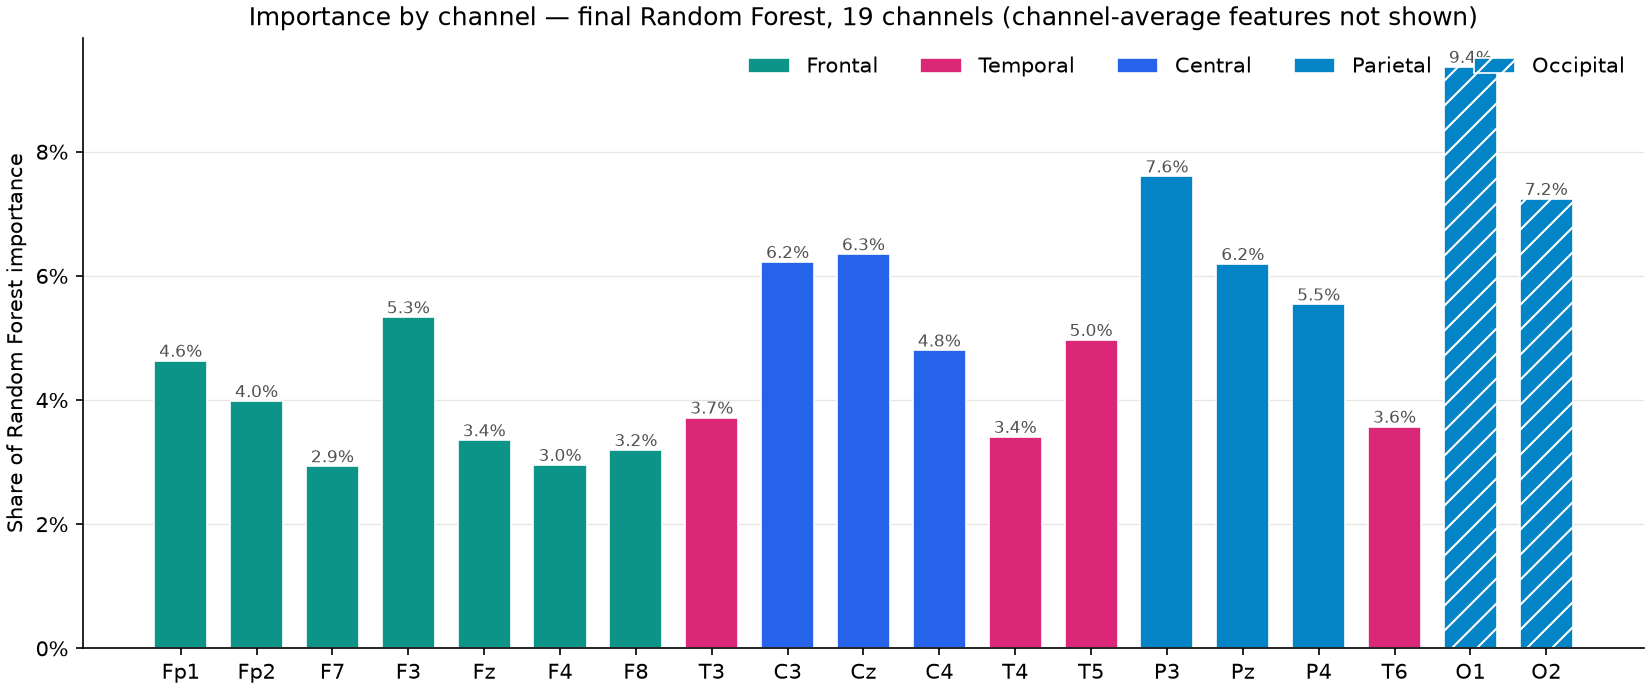
\includegraphics[width=0.95\linewidth]{official/channels/importance_by_channel.png}
  \caption{Random Forest feature importance, summed per channel (the cross-channel average
    columns are excluded here, to show per-channel differences clearly).}
  \label{fig:channel-importance}
\end{figure}

The occipital channels, O1 and O2, carry noticeably more importance than any other single
channel (9.4\% and 7.2\% of the total, respectively), with the parietal channels P3 and Pz
close behind. The frontal channels, by contrast, carry the least importance individually,
despite there being more of them. No channel dominates outright --- the heaviest single channel
still accounts for under 10\% of the total importance --- which is consistent with absence
seizures being a generalized, whole-scalp pattern rather than one localized to a single
electrode.

\begin{summarybox}
A 4th-order, zero-phase Butterworth band-pass filter (0.5--40~Hz) cleans drift and mains hum
without shifting seizure timing. The cleaned signal is cut into 31{,}419 windows of 2 seconds
with 50\% overlap, of which only 1{,}244 (3.96\%) contain a seizure --- the central imbalance
problem the rest of the classical pipeline has to deal with. Each window is reduced to 320
hand-crafted features: 8 time-domain and 8 frequency-domain feature types, each computed across
19 channels plus a cross-channel average.
\end{summarybox}

\chapter{Classical Machine Learning}
\label{chap:classicalml}

Twelve models were trained on the 320-feature dataset built in \Cref{chap:preprocessing}: four
algorithms, each trained three different ways. This chapter covers the algorithms, the training
modes, how a detection is scored, and these first 12 results, which were the project's baseline
for a long time. A later, wider search over augmentation methods (\Cref{chap:augmentation})
found a thirteenth model that beats every one of these --- that result is reported in full
there, not retrofitted into this chapter's original comparison.

\section{Four algorithms}

\begin{itemize}[leftmargin=1.4em]
  \item \textbf{Decision Tree} --- \texttt{DecisionTreeClassifier}, no feature scaling, default
    hyperparameters (Gini impurity, no depth limit).
  \item \textbf{Random Forest} --- \texttt{RandomForestClassifier}, no feature scaling, default
    hyperparameters (100 trees, no depth limit).
  \item \textbf{KNN} --- features standardized first, then \texttt{KNeighborsClassifier} with
    default settings (5 neighbors, uniform weighting).
  \item \textbf{SVM} --- features standardized first, then an RBF-kernel \texttt{SVC} with
    default settings (\(C = 1\), \(\gamma = \)~``scale''), with Platt scaling enabled so the
    model also outputs a calibrated probability. Platt scaling only adds this probability
    output; it does not change the underlying decision boundary.
\end{itemize}

All four pipelines use scikit-learn 1.9.1 with a fixed random seed (42) for reproducibility.
Random Forest and SVM are trained with default hyperparameters deliberately: the goal of this
project was a sound pipeline and an honest comparison across algorithms and training strategies,
not a hyperparameter search, which is left as future work (\Cref{chap:conclusion}).

\section{Three training modes}

Each of the four algorithms is trained three different ways, to address the class imbalance
established in \Cref{chap:preprocessing} head-on:

\begin{itemize}[leftmargin=1.4em]
  \item \textbf{Unbalanced.} Each training fold is used exactly as it is, with the real,
    heavily imbalanced class proportions.
  \item \textbf{Balanced.} The majority (non-seizure) class in the training fold is randomly
    undersampled down to match the seizure class, 50/50. This is repeated with 5 different
    random seeds to check how much the result depends on which non-seizure windows happen to
    get kept; seed 0 is the one used for the saved models and predictions reported below.
  \item \textbf{Augmented.} The full, unbalanced training fold, plus synthetic extra seizure
    windows built from the training recordings' own real signal. This mode is covered in detail
    in \Cref{chap:augmentation}.
\end{itemize}

In every mode, the test data is left untouched: real class proportions, real windows only, never
anything synthetic or resampled.

\section{How a detection is scored}

All 12 models are evaluated with a 5-fold \texttt{GroupKFold} split by recording, the same five
folds throughout this project: a model is never scored on a recording it was trained on. This
matters because neighboring windows from the same recording are highly correlated; splitting at
random, window by window, would let a model see near-duplicates of its test data during
training.

Scoring itself is event-level, not window-level. A window counts as positive once its predicted
probability crosses a chosen threshold; consecutive positive windows merge into one detected
interval, and nearby intervals (less than 2 seconds apart) are merged together, with anything
shorter than 2 seconds afterwards dropped as noise. A real seizure counts as \emph{found} if any
detected interval overlaps it at all; a detected interval that overlaps no real seizure counts
as a \emph{false alarm}.

\begin{figure}[H]
  \centering
  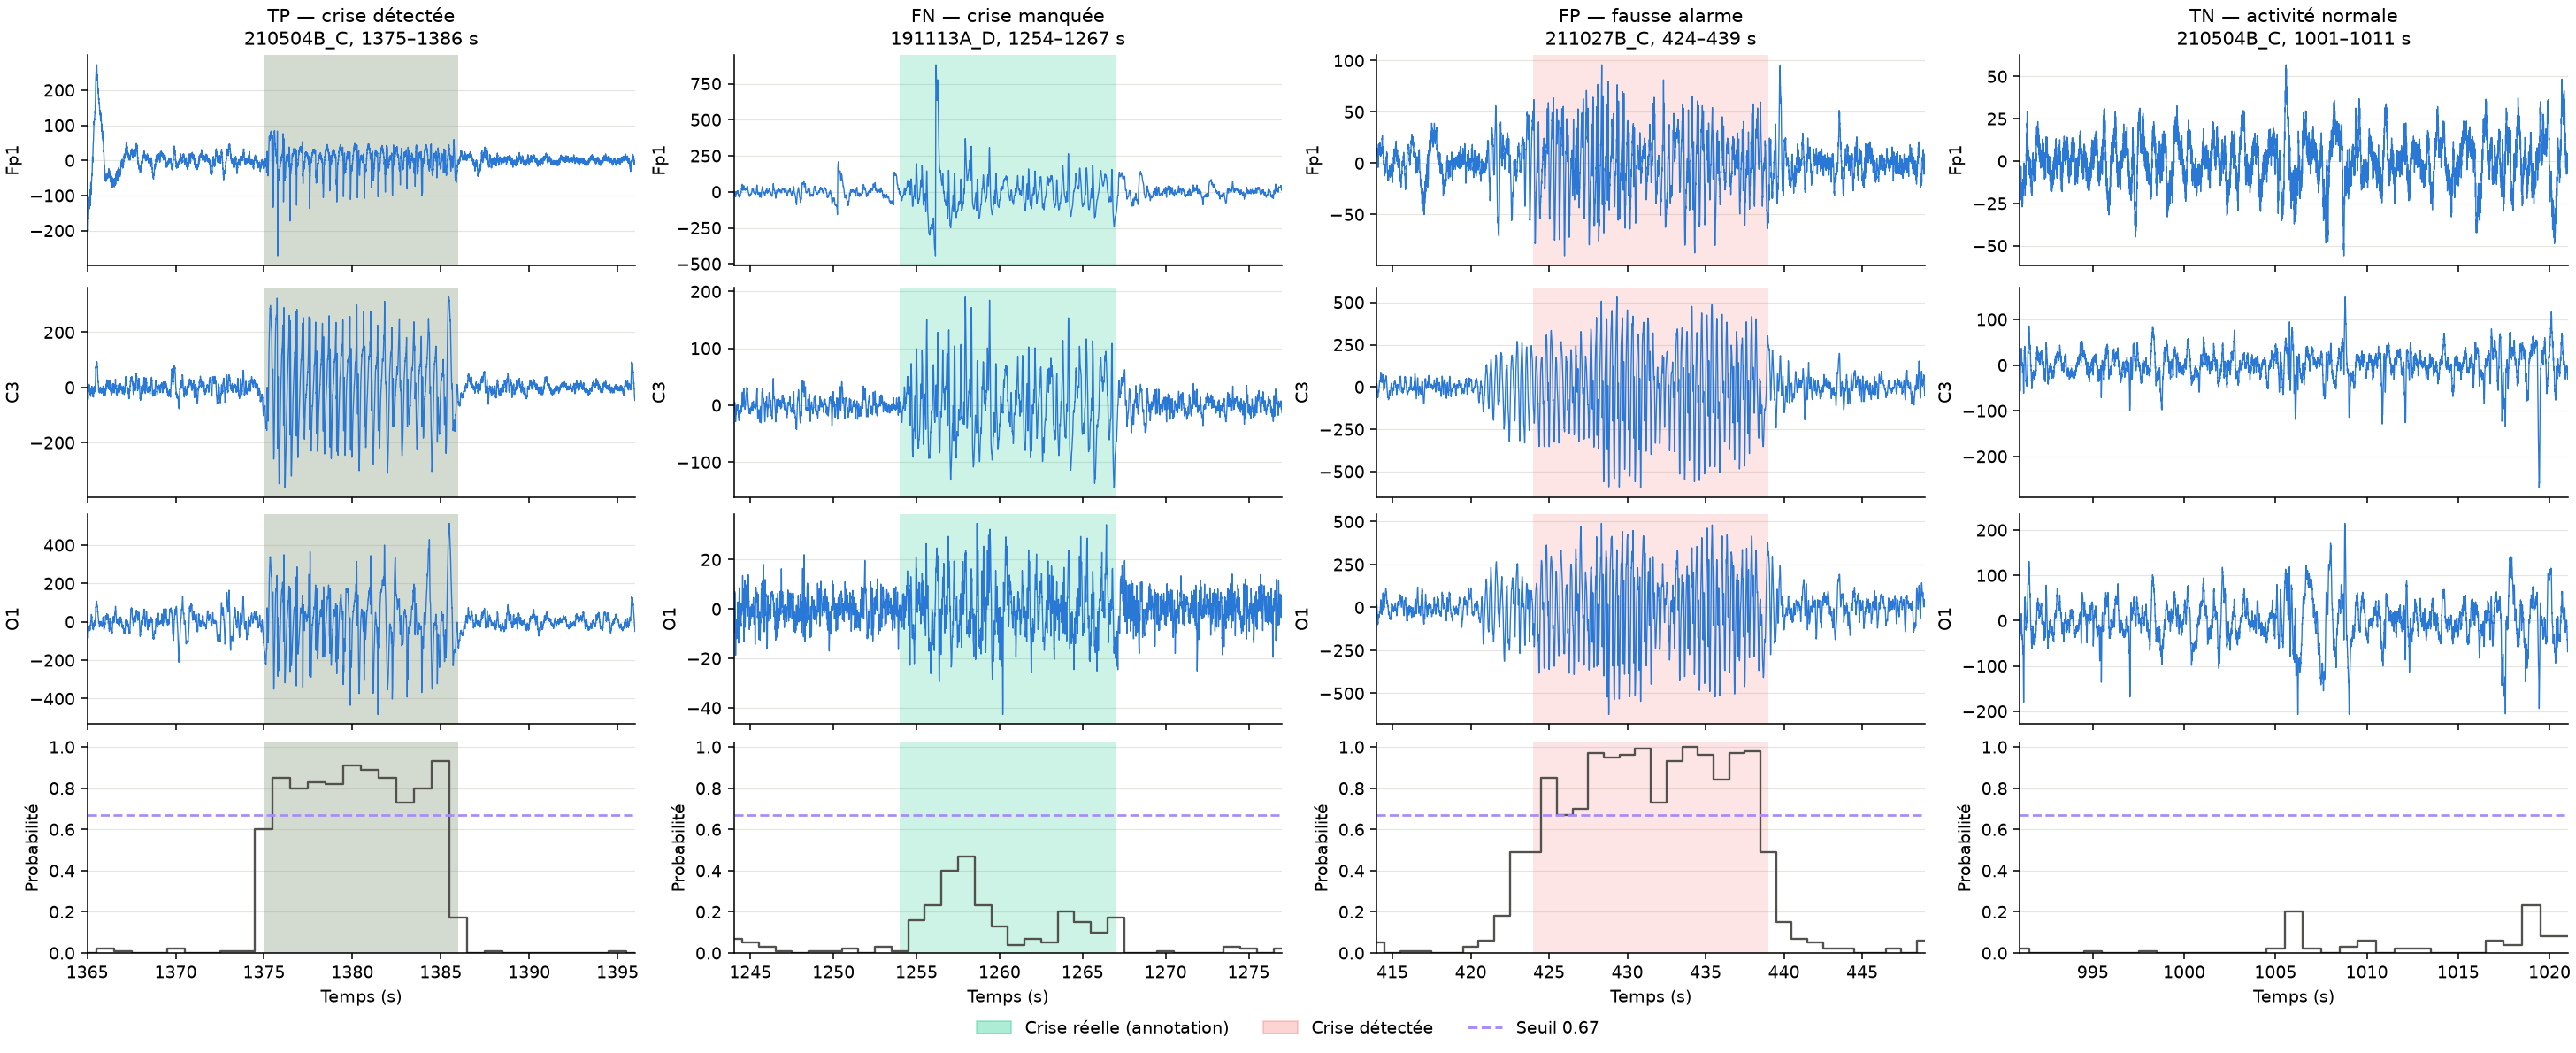
\includegraphics[width=\linewidth]{official/detection/error_examples.png}
  \caption{Four real 15-second segments from the Random Forest unbalanced model, one per
    outcome: a found seizure (TP, true positive), a missed seizure (FN, false negative), a
    false alarm (FP, false positive), and ordinary background activity correctly left alone
    (TN, true negative). Three EEG channels (Fp1, C3, O1) and the model's probability curve are
    shown for each; the dashed line is the detection threshold. Figure labels are in French in
    the original output (\emph{crise détectée} = seizure detected, \emph{crise manquée} =
    seizure missed, \emph{fausse alarme} = false alarm, \emph{activité normale} = normal
    activity, \emph{seuil} = threshold).}
  \label{fig:error-examples}
\end{figure}

The missed-seizure example is a useful reminder of what ``found'' actually requires: in that
segment, the model's probability does rise during the real seizure, but never crosses the
threshold --- a near miss, not a blind spot, and a case where a slightly lower threshold would
have caught it at the cost of more false alarms elsewhere, the exact trade-off the threshold
sweep in \Cref{chap:classicalml} is built to navigate.

Window-level accuracy is not used to judge these models: a model that never predicts a seizure
at all would still score 96\% window accuracy on this dataset, simply because seizure windows
are so rare. Event-level precision, recall, and F1 are the metrics used throughout this report.

For each model, a threshold is swept to find the one that maximizes event-level F1 on that
model's own out-of-fold predictions. Because the same predictions are used both to choose the
threshold and to score it, this ``best threshold'' number is slightly optimistic --- a caveat
carried through to \Cref{chap:evaluation}, where it matters for comparing fairly against the
deep-learning results.

\section{Results}

\Cref{tab:classical-results} gives every model's result at its own best threshold.

\begin{table}[H]
  \centering
  \small
  \caption{All 12 classical models, scored event-by-event at each model's own best threshold.
    FA = false alarms; FA/h = false alarms per hour of recording.}
  \label{tab:classical-results}
  \begin{tabular}{llrrrrrr}
    \toprule
    Algorithm & Mode & Thr. & Event F1 & Recall & Precision & Found/93 & FA (FA/h) \\
    \midrule
    Decision Tree & unbalanced & 0.05 & 0.290 & 0.978 & 0.170 & 91 & 561 (64.2) \\
    Decision Tree & balanced   & 0.05 & 0.148 & 0.989 & 0.080 & 92 & 1229 (140.7) \\
    Decision Tree & augmented  & 0.05 & 0.171 & 0.989 & 0.094 & 92 & 1007 (115.3) \\
    Random Forest & unbalanced & 0.67 & 0.867 & 0.935 & 0.807 & 87 & 26 (3.0) \\
    Random Forest & balanced   & 0.99 & 0.785 & 0.860 & 0.721 & 80 & 39 (4.5) \\
    Random Forest & augmented  & 0.93 & 0.854 & 0.903 & 0.810 & 84 & 26 (3.0) \\
    KNN & unbalanced & 0.61 & 0.828 & 0.925 & 0.750 & 86 & 37 (4.2) \\
    KNN & balanced   & 0.81 & 0.519 & 0.968 & 0.355 & 90 & 189 (21.6) \\
    KNN & augmented  & 0.81 & 0.692 & 0.968 & 0.539 & 90 & 95 (10.9) \\
    \textbf{SVM} & \textbf{unbalanced} & \textbf{0.82} & \textbf{0.894} & 0.925 & 0.866 &
      \textbf{86} & \textbf{16 (1.8)} \\
    SVM & balanced   & 0.99 & 0.821 & 0.860 & 0.785 & 80 & 29 (3.3) \\
    SVM & augmented  & 0.98 & 0.862 & 0.968 & 0.778 & 90 & 32 (3.7) \\
    \bottomrule
  \end{tabular}
\end{table}

The Decision Tree is a special case: it only ever outputs a probability of exactly 0 or 1, so
sweeping the threshold has no effect on its results.

\textbf{SVM, unbalanced training, is the best model among these original 12}: event F1 0.894, 86
of 93 seizures found, 16 false alarms (1.8 per hour), at a threshold of 0.82. It is the baseline
the rest of this report measures against. Random Forest unbalanced is a close second (F1 0.867);
the gap between the top two corresponds to only a handful of events and is not large enough to
call one algorithm definitively better than the other. The Decision Tree is, by a wide margin,
the weakest algorithm --- too unstable on a dataset with this few seizures and this much
imbalance. (A later model, built with an augmentation method evaluated in
\Cref{chap:augmentation}, overtakes this SVM and becomes the project's new default model; it is
not one of these original 12.)

\section{Balanced training: more seizures found, more mistakes made}

Balanced training raises recall for some models but lowers overall event F1 across the board: it
finds slightly more seizures while flooding the output with many more false alarms, because
undersampling changes the probabilities the model outputs in a way that is poorly calibrated
once evaluated back on the real, imbalanced test data. The best balanced-mode thresholds sit at
0.98--0.99, far higher than the unbalanced models' thresholds --- a direct symptom of this
miscalibration.

Repeating balanced training over 5 random seeds shows it is also less stable than unbalanced
training: SVM balanced's event F1 across seeds is \(0.797 \pm 0.017\), and Random Forest
balanced's is \(0.808 \pm 0.033\) --- noticeably more spread than the single, deterministic
unbalanced result.

\section{Are the false alarms really all mistakes?}

Not necessarily. For the best model of this original 12-model comparison (SVM, unbalanced), its
16 false alarms were checked against
the auxiliary signals and notes described in \Cref{chap:rawdata}: 7 of them (44\%) occur during
hyperpnea, a seizure-provocation technique that only covers 27.8\% of total recorded time; 1 of
them (6\%) during an SLI stimulation marker; and 2 of them (12\%) within 10 seconds of a
technician's own seizure-related note. Real, annotated seizures show the same pull toward
hyperpnea (37 of 93, 40\%) --- unsurprising, since hyperpnea exists specifically to provoke
them. This does not prove any particular false alarm is secretly a real, unannotated seizure,
but it is consistent with that possibility, and it is the reason a neurologist's review of these
false alarms is listed as future work in \Cref{chap:conclusion}.

\begin{figure}[H]
  \centering
  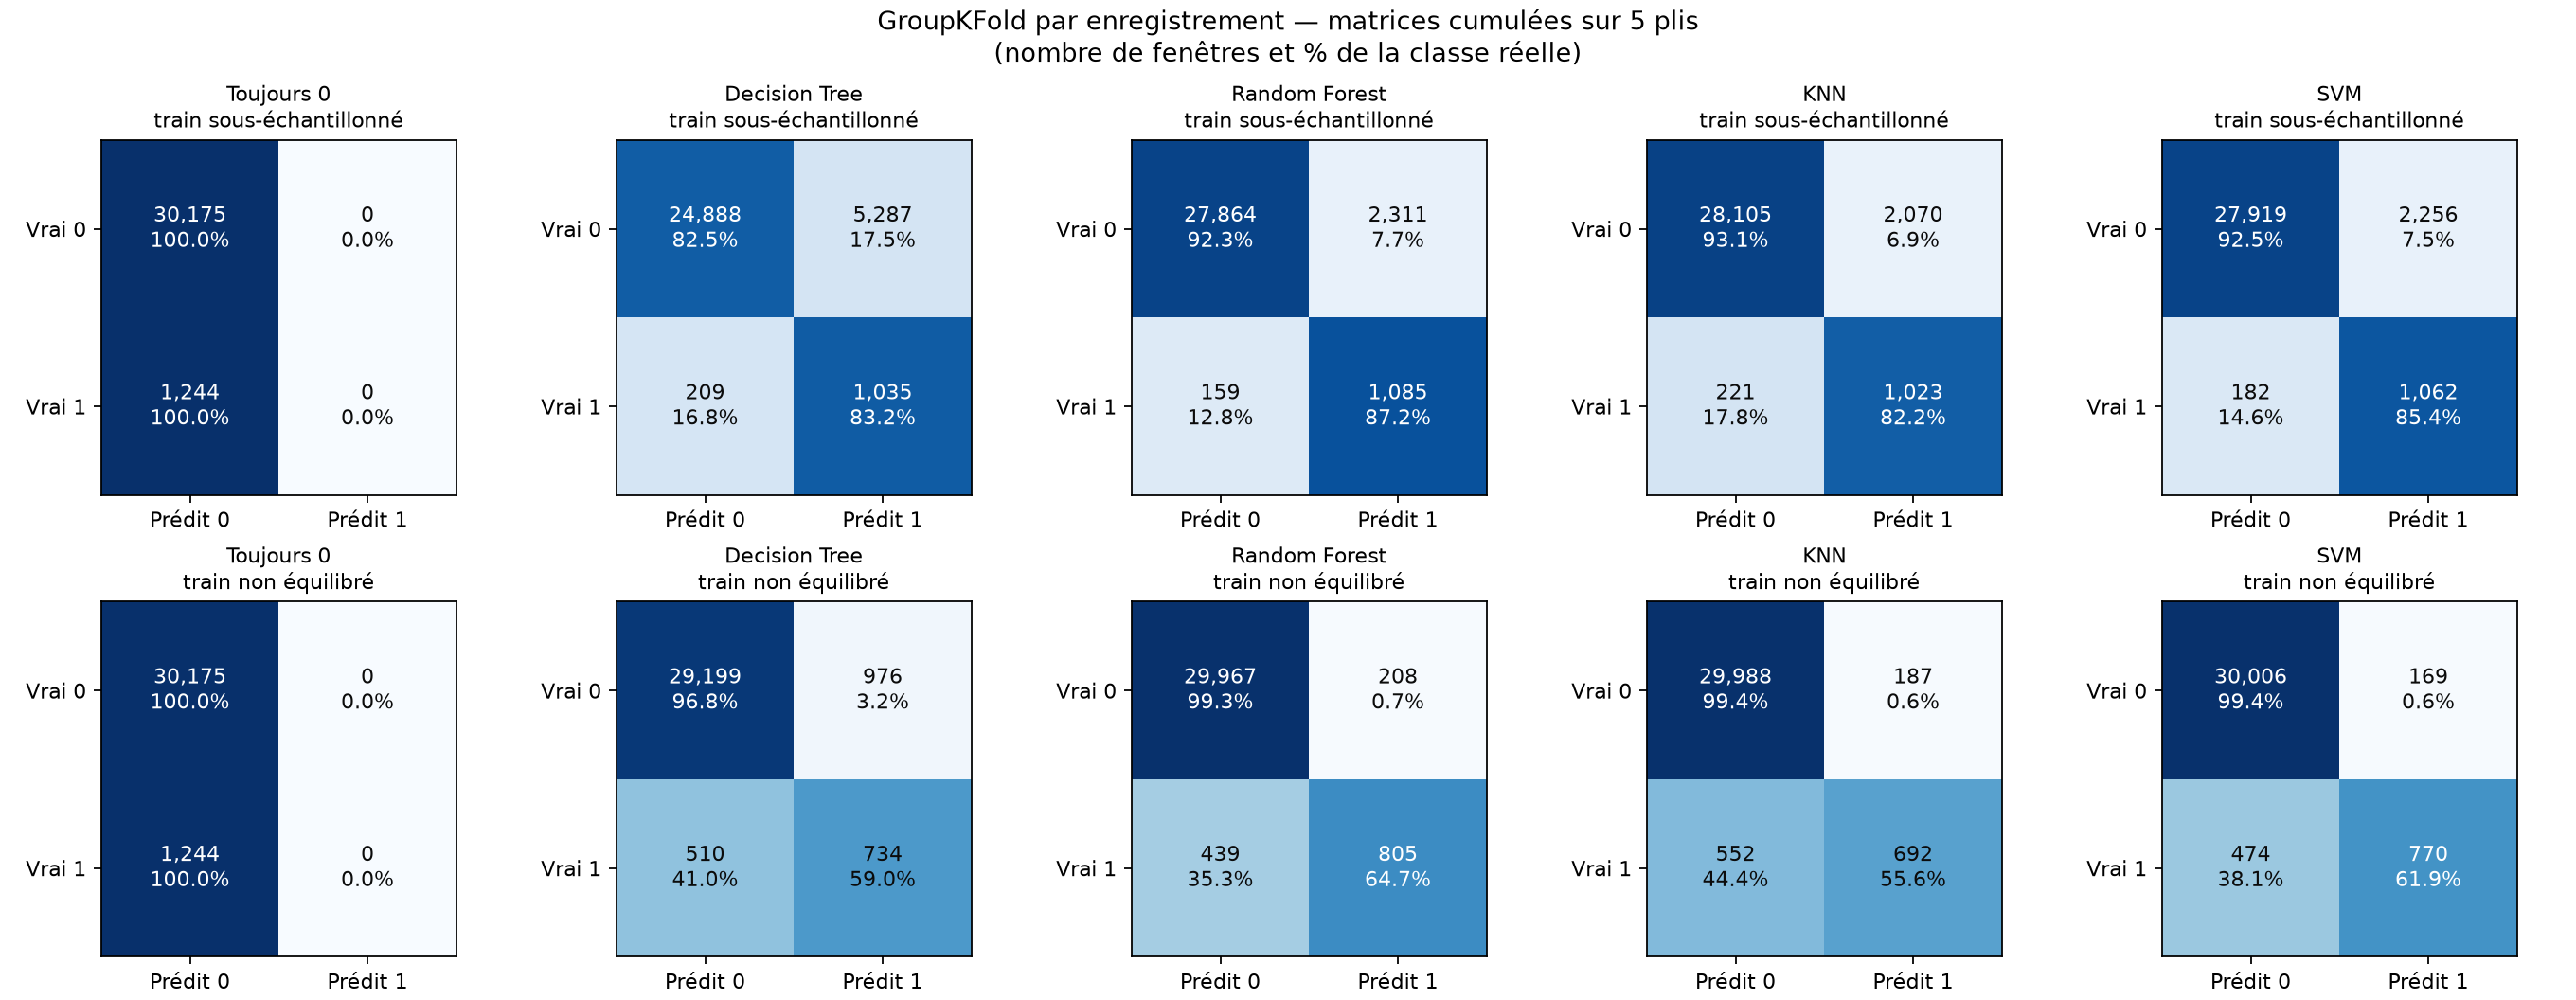
\includegraphics[width=0.95\linewidth]{official/models/confusion_matrices_groupkfold.png}
  \caption{Window-level confusion matrices for the 12 models under the \texttt{GroupKFold}
    protocol used throughout this report.}
  \label{fig:confusion-matrices}
\end{figure}

\begin{summarybox}
Twelve models --- Decision Tree, Random Forest, KNN, and SVM, each trained unbalanced, balanced,
and augmented --- were scored event by event with a recording-level 5-fold split. SVM,
unbalanced, is the best single model: event F1 0.894, 86 of 93 seizures found, 16 false alarms.
Balanced training raises recall slightly but adds far more false alarms, hurting overall F1 and
proving less stable across random seeds. A look at the best model's false alarms shows a
meaningful fraction coincide with hyperpnea or technician notes --- a real, open question about
whether some are actually unannotated seizures.
\end{summarybox}

\chapter{Data Augmentation}
\label{chap:augmentation}

The first augmentation attempt (shift and mirror) never beat the plain baseline. Rather than
stop there, five more methods were tried, each tested alone first, then the winners combined
--- and one of them turned out to be the best single model in the entire project. This chapter
covers all six methods, why each one was chosen, and the full, honest result of testing them.

\section{Shift and mirror: the first attempt}

Only seizure (class 1) windows are created, and only from the real, filtered signal of the
training recordings --- never from recordings held out for testing, and never anything
synthesized from nothing.

\begin{itemize}[leftmargin=1.4em]
  \item \textbf{Shift.} Extra 2-second windows starting 0.25, 0.5, and 0.75 seconds after each
    regular window's start time (the regular window grid has a 1-second hop), kept under the
    same rule used everywhere else: at least 50\% seizure coverage.
  \item \textbf{Mirror.} Every seizure window, regular or shifted, with its left and right
    electrodes swapped: Fp1$\leftrightarrow$Fp2, F7$\leftrightarrow$F8, F3$\leftrightarrow$F4,
    T3$\leftrightarrow$T4, C3$\leftrightarrow$C4, T5$\leftrightarrow$T6, P3$\leftrightarrow$P4,
    O1$\leftrightarrow$O2. The three midline channels, Fz, Cz, and Pz, are left unchanged.
\end{itemize}

Across the 21 recordings this adds 8{,}230 synthetic seizure windows on top of the 1{,}244
original ones: 3{,}493 shifted, 1{,}244 mirrored, and 3{,}493 both shifted and mirrored. These
were chosen first because both stay entirely inside real, recorded signal --- nothing is
synthesized, so nothing physiologically implausible can be fabricated by the transformation
itself. Mirroring is anatomically justified specifically for absence seizures (generalized,
bilaterally synchronous discharges, so a left-right-swapped window is still a valid seizure
pattern); shifting is consistent with a tolerance already built into the official labeling rule.

The result, reported honestly: shift+mirror raised recall for every algorithm (SVM: 86 to 90 of
93 found) but also raised false alarms sharply (SVM: 16 to 32) and lowered event F1 (SVM: 0.894
to 0.862). It never beat the plain, unbalanced baseline for any of the four algorithms.

\section{Five more methods, tried the same way}

A negative result for one method is not a verdict on augmentation in general. Five more
methods were built, each respecting the same rule as shift and mirror --- training folds only,
built from real signal, one new synthetic window per real seizure window (no extra time
offsets, so each method adds exactly 1{,}244 windows, directly comparable to one another):

\begin{itemize}[leftmargin=1.4em]
  \item \textbf{Amplitude scaling.} Multiply the whole window by a random gain between 0.6 and
    1.6, simulating the kind of electrode-to-electrode or session-to-session gain variation a
    real recording can have.
  \item \textbf{Noise.} Add Gaussian noise to the window, scaled to that window's own signal
    level, simulating ordinary sensor noise.
  \item \textbf{Time masking.} Blank out a short random contiguous span inside the window (up to
    25\% of it) to zero, forcing the model not to rely on any one instant.
  \item \textbf{Channel dropout.} Zero out 1 to 3 random EEG channels for the whole window,
    simulating electrodes that failed or were never connected.
  \item \textbf{Combined.} The windows from whichever of the above turned out to help, merged
    into one dataset --- built only after the individual results were in, not before.
\end{itemize}

The broader menu of EEG augmentation methods also includes frequency-domain transforms (Fourier
surrogates, frequency shift), mixing methods (mixup, cutmix, pasting segments), and generative
models (GANs, VAEs, diffusion). These were set aside for the same reason shift and mirror were
originally preferred over them: generative methods need far more than 93 seizures to avoid
memorizing or fabricating unrealistic signal, and mixing methods risk blending two unrelated
seizure segments into a composite that does not correspond to any real physiological event. The
five methods above were chosen because each one models a specific, plausible real-world
imperfection (gain drift, sensor noise, a dead channel, a brief dropout) rather than an
arbitrary transformation.

\section{What actually helped}

\begin{table}[H]
  \centering
  \small
  \caption{Every augmentation method, every algorithm, event F1 at its own best threshold.
    Bold marks the best result for that algorithm; a dagger marks a result that beats the
    algorithm's own unbalanced baseline.}
  \label{tab:augmentation-full}
  \begin{tabular}{llrrr}
    \toprule
    Algorithm & Method & Event F1 & Found/93 & False alarms \\
    \midrule
    SVM & unbalanced (baseline) & 0.894 & 86 & 16 \\
    SVM & shift + mirror & 0.862 & 90 & 32 \\
    SVM & amplitude & 0.882 & 88 & 23 \\
    SVM & noise & 0.889 & 87 & 20 \\
    SVM & time masking & 0.870 & 87 & 25 \\
    SVM & \textbf{channel dropout} & \textbf{0.901}$^\dagger$ & 88 & 18 \\
    SVM & combined (noise + dropout) & 0.889 & 87 & 20 \\
    \midrule
    Random Forest & unbalanced (baseline) & 0.867 & 87 & 26 \\
    Random Forest & shift + mirror & 0.854 & 84 & 26 \\
    Random Forest & amplitude & 0.867 & 87 & 24 \\
    Random Forest & noise & 0.872$^\dagger$ & 86 & 23 \\
    Random Forest & time masking & 0.859 & 79 & 15 \\
    Random Forest & \textbf{channel dropout} & \textbf{0.880}$^\dagger$ & 82 & 14 \\
    Random Forest & combined (noise + dropout) & 0.878$^\dagger$ & 81 & 13 \\
    \midrule
    KNN & unbalanced (baseline) & 0.828 & 86 & 37 \\
    KNN & \textbf{noise} & \textbf{0.832}$^\dagger$ & 81 & 29 \\
    KNN & combined (noise + dropout) & 0.829$^\dagger$ & 81 & 30 \\
    \midrule
    Decision Tree & unbalanced (baseline) & 0.290 & 91 & 561 \\
    Decision Tree & \textbf{combined (noise + dropout)} & \textbf{0.296}$^\dagger$ & 93 & 619 \\
    Decision Tree & noise & 0.295$^\dagger$ & 93 & 570 \\
    \bottomrule
  \end{tabular}
\end{table}

Two methods actually work: \textbf{channel dropout} and \textbf{noise}. Channel dropout gives
the single best result in this entire project --- SVM with channel-dropout augmentation reaches
event F1 \textbf{0.901} (88 of 93 found, 18 false alarms, threshold 0.90), beating the plain SVM
baseline (0.894) by the same margin the much more expensive SVM+CNN ensemble achieved
(\Cref{chap:ensemble}), except this is one plain model, not a blend of two. Channel dropout also
helps Random Forest (0.867 to 0.880). Noise helps Random Forest, KNN, and (marginally)
Decision Tree.

Time masking hurt every algorithm it was tried on, and amplitude scaling was mixed (helped SVM,
did nothing for Random Forest). Combining the two winners, noise and channel dropout, into one
dataset did \emph{not} beat channel dropout alone for either SVM (0.889 vs.\ 0.901) or Random
Forest (0.878 vs.\ 0.880) --- the single best method outperformed the combination, a useful
reminder that more augmentation is not automatically better augmentation.

\textbf{Why channel dropout specifically works}: \Cref{chap:preprocessing} showed that no single
EEG channel dominates a trained model's decisions (the heaviest channel, O1, carries under 10\%
of total importance), consistent with absence seizures being a generalized, whole-scalp pattern.
Channel dropout trains the model on windows missing 1--3 channels, which cannot destroy the
seizure signature --- plenty of real signal remains in the other 16--18 channels. Time masking,
by contrast, removes a slice of \emph{every} channel at the same instant, which can erase the
one thing that actually identifies an absence seizure: its rhythm over time. Losing space is
survivable for this problem; losing time is not.

\begin{summarybox}
Six augmentation methods were tried: the original shift+mirror, four new methods tested in
isolation (amplitude scaling, noise, time masking, channel dropout), and one combined dataset
built from the two methods that actually helped. Only channel dropout and noise improved
results; channel dropout gives the best result in the whole project, SVM at event F1 0.901,
beating the plain SVM baseline (0.894) as a single model, no blending required. Combining the
two winners did not beat the best one alone. Time masking consistently hurt, and the original
shift+mirror method never beat the baseline for any algorithm --- a real negative result,
reported alongside the real positive one.
\end{summarybox}

\chapter{Ensemble}
\label{chap:ensemble}

Many models already exist, fully trained, each producing an out-of-fold probability for every
window. Rather than train anything new, this chapter asks a cheaper question: does simply
averaging the probabilities of two or more already-trained models do better than the best one
alone?

\section{Method}

Each ensemble blends the out-of-fold probabilities of two or more already-trained models (and,
in several rows below, one CNN) by averaging them --- no retraining involved. Two different
threshold conventions are reported, because they answer different questions:

\begin{itemize}[leftmargin=1.4em]
  \item \textbf{Held-out-fold} (the honest number): for each of the 5 outer folds, the detection
    threshold is swept using only the \emph{other} four folds' predictions, never the fold being
    scored.
  \item \textbf{Optimistic}: a single threshold swept across all out-of-fold predictions at
    once --- the same convention used for the ``best threshold'' column in
    \Cref{tab:classical-results}, kept here only for comparison.
\end{itemize}

\section{Results}

\begin{table}[H]
  \centering
  \small
  \caption{Ensemble blends, held-out-fold threshold, against the two single-model baselines.}
  \label{tab:ensemble-results}
  \begin{tabular}{p{6.4cm}rrrr}
    \toprule
    Ensemble & Event F1 & Found/93 & FA & SzCORE F1 \\
    \midrule
    SVM, channel dropout (single model, new best) & \textbf{0.901} & 88 & 18 & --- \\
    SVM Unbalanced (single model, original baseline) & 0.894 & 86 & 16 & --- \\
    SVM Unbalanced + ShallowConvNet Augmented & 0.901 & 90 & 19 & 0.900 \\
    SVM, channel dropout + ShallowConvNet, amplitude & 0.896 & 89 & 19 & 0.892 \\
    SVM Unbalanced + Random Forest Unbalanced & 0.894 & 85 & 15 & 0.894 \\
    SVM, channel dropout + Random Forest Unbalanced & 0.823 & 84 & 31 & 0.866 \\
    SVM, channel dropout + Random Forest, channel dropout & 0.817 & 81 & 29 & 0.846 \\
    SVM Unb.\ + RF Unb.\ + KNN Unb. & 0.874 & 83 & 18 & 0.881 \\
    SVM Unbalanced + KNN Unbalanced & 0.871 & 81 & 15 & 0.872 \\
    2$\times$SVM Unb.\ + Random Forest Unb. & 0.849 & 83 & 23 & 0.870 \\
    \bottomrule
  \end{tabular}
\end{table}

\textbf{No ensemble beats the best single model.} SVM with channel-dropout augmentation
(\Cref{chap:augmentation}) reaches event F1 0.901 on its own. The best ensemble found, SVM
Unbalanced blended with the augmented ShallowConvNet CNN, reaches exactly the same score, 0.901
--- a genuine tie, not an improvement, and it does so with a different, more expensive recipe (a
second model to train and maintain) for the same result a single classical model already gives.

Blending the \emph{new} best SVM with anything else actually makes things worse, not better:
paired with the best CNN it drops to 0.896; paired with Random Forest (either version) it drops
further, to 0.817--0.823. This makes sense in hindsight --- the earlier ensemble gains came from
combining models that made \emph{different kinds} of mistakes (SVM unbalanced is conservative
and precise, the CNN and Random Forest catch different seizures). The new best SVM already
captures much of that diversity internally, through the channel-dropout training itself, so
blending it with another model adds noise more than it adds new information.

The older SVM+Random Forest blend (both unbalanced) still ties the original 0.894 baseline, with
a different mix of hits and misses (85 found, 15 false alarms, against the SVM alone's 86 and
16) --- a result worth remembering but not a reason to prefer it over either single-model result
above.

\begin{summarybox}
Blending already-trained models, with no retraining, was tried extensively. The best blend found
(SVM unbalanced + an augmented CNN) ties the project's best single model (0.901) but never beats
it, and blending the new best SVM (channel-dropout augmentation) with anything else makes results
worse. The practical conclusion: a single, well-chosen model --- SVM with channel-dropout
augmentation --- is both the simplest and the best-performing option in this project, with no
ensemble complexity needed to reach the same score.
\end{summarybox}

\chapter{Deep Learning}
\label{chap:deeplearning}

Every model in \Cref{chap:classicalml} learns from 320 hand-crafted features. This chapter asks
whether a model that instead learns directly from the raw, filtered signal can do better ---
trained on a separate GPU machine, since the classical pipeline's CPU-only environment has no
PyTorch installed, and scored back here under the same event-level rules as everything else.

\section{Two architectures}

Two compact convolutional architectures were trained, both standard, well-established choices
for EEG decoding rather than custom designs:

\begin{itemize}[leftmargin=1.4em]
  \item \textbf{ShallowConvNet}: a temporal convolution followed by a spatial convolution and
    pooling --- a simple, well-tested baseline architecture for EEG classification.
  \item \textbf{EEGNet}: a compact network built from depthwise and separable convolutions,
    designed specifically to be parameter-efficient on small EEG datasets.
\end{itemize}

Both are deliberately small, with only a few thousand parameters each. With 93 seizures in
total, a larger network would risk simply memorizing the training recordings rather than
learning a general seizure pattern.

\section{Input and training recipe}

Each input is 4 seconds of all 19 filtered EEG channels (1{,}024 samples at 256~Hz), centered on
one of the official 2-second windows, so every CNN prediction lines up with exactly the same
window the classical models were scored on. Each recording is normalized per channel using a
robust statistic, the median and the median absolute deviation, clipped at $\pm 20$, rather than
a plain mean and standard deviation, to reduce the influence of large artifacts.

Training uses the same 5 outer \texttt{GroupKFold} folds as the classical models. Within each
outer fold, some training recordings are further held out for early stopping and for choosing
that fold's detection threshold, so the test fold is never touched during training or threshold
selection. The real, imbalanced class proportions are kept; a weighted cross-entropy loss
up-weights the seizure class to counter the imbalance. Training uses AdamW with a cosine
learning-rate schedule, early stopping on validation average precision, and several random seeds
per fold, with the resulting probabilities averaged across seeds.

Optional online augmentation is applied to \emph{both} classes during training, generated fresh
on the fly per training batch rather than pre-built into a fixed extra dataset --- a
deliberately different strategy from the classical pipeline's augmentation in
\Cref{chap:augmentation}, which only ever touches the seizure class. Eight transforms are
available, each independently selectable so it can be tested alone or combined: the original
five (amplitude scaling, small added noise, channel dropout, left-right mirroring, small time
shifts) plus three more added for this project's wider augmentation sweep: time masking
(zeroing a short random span), frequency band-stop (suppressing a random 1--4~Hz band), and
mixup (linearly blending two windows and their labels).

\section{A real bug: the IndexError in \texttt{event\_counts()}}

During development, the CNN training script crashed with
\texttt{IndexError: index 7943 is out of bounds for axis 0 with size 4344}. The cause: the
function responsible for counting detected events per recording, \texttt{event\_counts()}, used
the \emph{labels} returned by a pandas \texttt{groupby(...).groups} dictionary as if they were
array \emph{positions}. This happens to work only when a table's row index is untouched,
running from 0 to its length minus one. It silently broke the moment the function was handed a
validation subset sliced out of a larger table with \texttt{.iloc[]}, because that subset keeps
its original row numbers rather than renumbering from zero --- and it crashed specifically when
a randomly chosen validation recording's original row number happened to exceed the size of the
smaller validation subset. Earlier runs had not hit this because, by luck, the recordings chosen
for validation had not triggered it.

The fix computes the recording labels, interval starts, and interval ends as plain arrays once,
then selects rows with a boolean mask instead of looking anything up by index label --- correct
regardless of how the table was sliced beforehand. This is the kind of bug that is easy to miss
in testing and only shows up on certain random splits, which is why it is called out here rather
than quietly fixed and forgotten.

\section{Results}

The first run tried the five original transforms only as one fixed combination. A later, wider
sweep tested every transform in isolation --- the same ``test each one alone, then combine the
winners'' approach used on the classical side (\Cref{chap:augmentation}) --- to see whether any
single transform could do better than the original combo, and whether the three new transforms
(time masking, band-stop, mixup) helped at all.

\begin{table}[H]
  \centering
  \small
  \caption{Every CNN run, ShallowConvNet unless noted, nested threshold (best of plain and
    smoothed+hysteresis). FA = false alarms.}
  \label{tab:cnn-results}
  \begin{tabular}{lrrr}
    \toprule
    Model & Event F1 & Found/93 & FA \\
    \midrule
    SVM, channel dropout (classical, new best) & \textbf{0.901} & 88 & 18 \\
    SVM, unbalanced (classical, original baseline) & 0.894 & 86 & 16 \\
    \midrule
    \textbf{Amplitude alone} & \textbf{0.817} & 77 & 19 \\
    Original five, combined (``augmented'') & 0.815 & 77 & 21 \\
    EEGNet, original five combined & 0.811 & 85 & 32 \\
    Mixup & 0.802 & 78 & 24 \\
    Mirror alone & 0.798 & 79 & 27 \\
    Time masking alone & 0.790 & 77 & 25 \\
    Time shift alone & 0.788 & 77 & 26 \\
    Plain (no augmentation) & 0.781 & 76 & 26 \\
    Noise alone & 0.778 & 76 & 27 \\
    Noise + time masking (combined) & 0.774 & 78 & 32 \\
    Band-stop alone & 0.774 & 76 & 28 \\
    Channel dropout alone & 0.767 & 76 & 30 \\
    \bottomrule
  \end{tabular}
\end{table}

None of the 12 CNN runs beats the classical models; the best of them, amplitude scaling alone,
falls 0.084 short of the new SVM best (0.901) and 0.077 short of the original SVM baseline
(0.894). This matches the expectation stated from the start of this project: 93 seizures spread
across 21 patients is too little data for a raw-signal convolutional network to out-learn
hand-designed features. It is recorded here as a real, useful finding, not a failure.

The isolated-transform sweep itself is a smaller, closer race: amplitude scaling alone
(0.817) \emph{barely} edges out the original five-transform combination (0.815) --- a
difference of 0.002, well within normal run-to-run noise, so this should be read as a tie, not a
win for isolating transforms. Unlike the classical pipeline, where channel dropout was a clear,
substantial winner once isolated, no single CNN transform stands out from the pack: most scores
cluster between 0.77 and 0.82 regardless of which transform is used, and combining noise with
time masking (0.774) did not beat either alone. Channel dropout, the classical pipeline's best
method, is actually the \emph{weakest} transform for the CNN (0.767) --- the opposite of what
happened with the feature-based models, a reminder that a transform's effect depends on how a
model is trained, not just on the transform itself.

Smoothing and hysteresis post-processing (described fully in \Cref{chap:evaluation}) was applied
to every CNN run; it helped most of them (plain: $+0.007$; amplitude: $+0.006$; mirror:
$+0.016$; and EEGNet's combo substantially, $+0.035$) but slightly hurt the original five-combo
run ($-0.004$) and time shift ($-0.027$). \Cref{tab:cnn-results} reports each model at whichever
of the two did better for it, which is also how the classical-vs-CNN comparison is framed
throughout this report.

\begin{summarybox}
Two compact CNNs, ShallowConvNet and EEGNet, were trained directly on 4-second raw EEG windows
on a separate GPU machine, under the same recording-level evaluation as the classical models. A
real bug --- an index-label-vs-position mix-up in the event-counting code --- caused a crash on
certain random splits and was fixed once understood. A full sweep of 8 augmentation transforms,
isolated and combined, found no single transform clearly better than the original five-transform
combo (amplitude alone edges it out by 0.002, within noise), and channel dropout --- the
classical pipeline's best method --- is actually the CNN's weakest. None of the 12 CNN runs
(best: 0.817) beats the classical SVM (0.894, or the new best, 0.901), the expected, documented
outcome for a raw-signal model trained on only 93 seizures.
\end{summarybox}

\chapter{Evaluation}
\label{chap:evaluation}

The preceding chapters all use event-level F1 (\Cref{chap:classicalml}), but not always under
exactly the same threshold-selection rule. This short chapter names the differences explicitly,
so the comparisons in this report are read correctly rather than taken at face value.

\section{Smoothing and hysteresis}

A second, optional detection path exists, applied with no retraining: the per-window
probabilities are first smoothed with a centered rolling median, then thresholded with
\emph{hysteresis} --- a higher threshold is needed to start a detected event, and a lower
threshold is enough to let an already-started event continue. This generally produces fewer,
cleaner intervals than thresholding the raw probabilities directly. It is applied automatically,
and reported alongside the plain result, for the CNN evaluations in \Cref{chap:deeplearning}; it
is \emph{not} applied to the 12 classical models' headline numbers in
\Cref{tab:classical-results}, which use the plain, unsmoothed path only. This is a real
methodological difference between the two chapters' numbers, named here so it is not mistaken
for an oversight.

\section{Three ways of choosing a threshold}

The ``best threshold'' reported for every classical model, including the augmentation sweep in
\Cref{chap:augmentation}, is chosen and scored on the same out-of-fold predictions, which makes
every classical headline number --- the original 0.894 and the new best, 0.901 --- slightly
optimistic. The ensemble results in \Cref{chap:ensemble} and the CNN results in
\Cref{chap:deeplearning} are more careful: each outer fold's threshold is chosen only from data
outside that fold (other folds, for the ensembles; held-out training recordings, for the CNNs),
never from the fold being scored.

A fully nested re-scoring of the classical models, under this same stricter rule, is not
finished --- only 3 models have been run this way so far (the full run is memory-heavy and was
interrupted once for lack of RAM), and none of them is the new best model (SVM, channel
dropout). Until it is, the comparison between the classical models' 0.894/0.901 and the best
CNN's 0.817 should be read as informative but not perfectly matched: the classical numbers carry
a small optimism the CNN numbers do not.

\section{Where this leaves the comparison}

\begin{table}[H]
  \centering
  \caption{The project's results, side by side, with the threshold protocol each one used.}
  \label{tab:final-comparison}
  \small
  \begin{tabular}{p{7.3cm}rl}
    \toprule
    Result & Event F1 & Threshold protocol \\
    \midrule
    \textbf{SVM, channel-dropout augmentation (best overall)} & \textbf{0.901} & same-fold (optimistic) \\
    SVM + ShallowConvNet ensemble (ties the best) & 0.901 & held-out-fold \\
    SVM, unbalanced (original baseline) & 0.894 & same-fold (optimistic) \\
    SVM + Random Forest ensemble (ties the original baseline) & 0.894 & held-out-fold \\
    ShallowConvNet, amplitude alone (best CNN) & 0.817 & nested \\
    \bottomrule
  \end{tabular}
\end{table}

Taken together: a single classical model, SVM trained with channel-dropout augmentation, is both
the simplest and the best-performing result in this project. Every attempt to do better by
blending models ties it at best, never beats it. The CNN, trained end-to-end on raw signal, does
not come close to the feature-engineered approach at this dataset size, no matter which of its 8
augmentation transforms is used --- exactly the outcome the project set out to test for.

\begin{summarybox}
Three threshold-selection rules are in play across this report --- same-fold (slightly
optimistic), held-out-fold, and nested --- and they are not interchangeable. The one piece of
evaluation work still missing is a full nested re-scoring of the classical models (including the
new best one), which would make the classical-vs-CNN comparison fully fair; until then, the
classical numbers should be read as slightly favorable to the classical side relative to the
CNNs' nested 0.817. Even allowing for that gap, the margin (0.901 vs.\ 0.817) is wide enough that
the conclusion --- classical beats deep learning here --- is not in doubt.
\end{summarybox}

\chapter{The Application}
\label{chap:application}

Every result in this report can also be explored directly, not just read off a table. A Dash
web application reads the recordings, the model predictions, and the evaluation results that
earlier steps already computed; it trains nothing itself. This chapter walks through it with
real screenshots, not mockups.

\section{Structure}

The application has four pages: \textbf{Home}, \textbf{Visualisation}, \textbf{Prediction}, and
\textbf{Comparison}.

\begin{itemize}[leftmargin=1.4em]
  \item \textbf{Home} explains the method in plain language for a first-time visitor: how the
    data was prepared, what each training mode means. The augmented mode, for instance, is
    described in the app itself as ``every training window plus extra seizure windows: shifted
    by 0.25 to 0.75~s and mirrored left-right'' --- the same transformation described in detail
    in \Cref{chap:augmentation}.
  \item \textbf{Visualisation} lets a visitor browse a recording's raw EEG signal directly, with
    channels grouped in the sidebar by scalp region (frontal, central, temporal, posterior)
    rather than listed alphabetically.
  \item \textbf{Prediction} overlays a chosen model's detected intervals on a recording's signal
    and its real annotated seizures, so a false alarm or a missed seizure can be inspected
    directly against the EEG around it.
  \item \textbf{Comparison} ranks the models against each other. Its ranking table supports 12
    different sort metrics --- event F1, recall, precision, seizures found, missed seizures,
    false alarms, false alarms per hour, window-level F1/recall/precision, onset/offset error,
    and training time --- so a visitor can re-rank the models by whichever criterion matters
    most to them, not only by F1.
\end{itemize}

\begin{figure}[H]
  \centering
  \begin{subfigure}[b]{0.48\linewidth}
    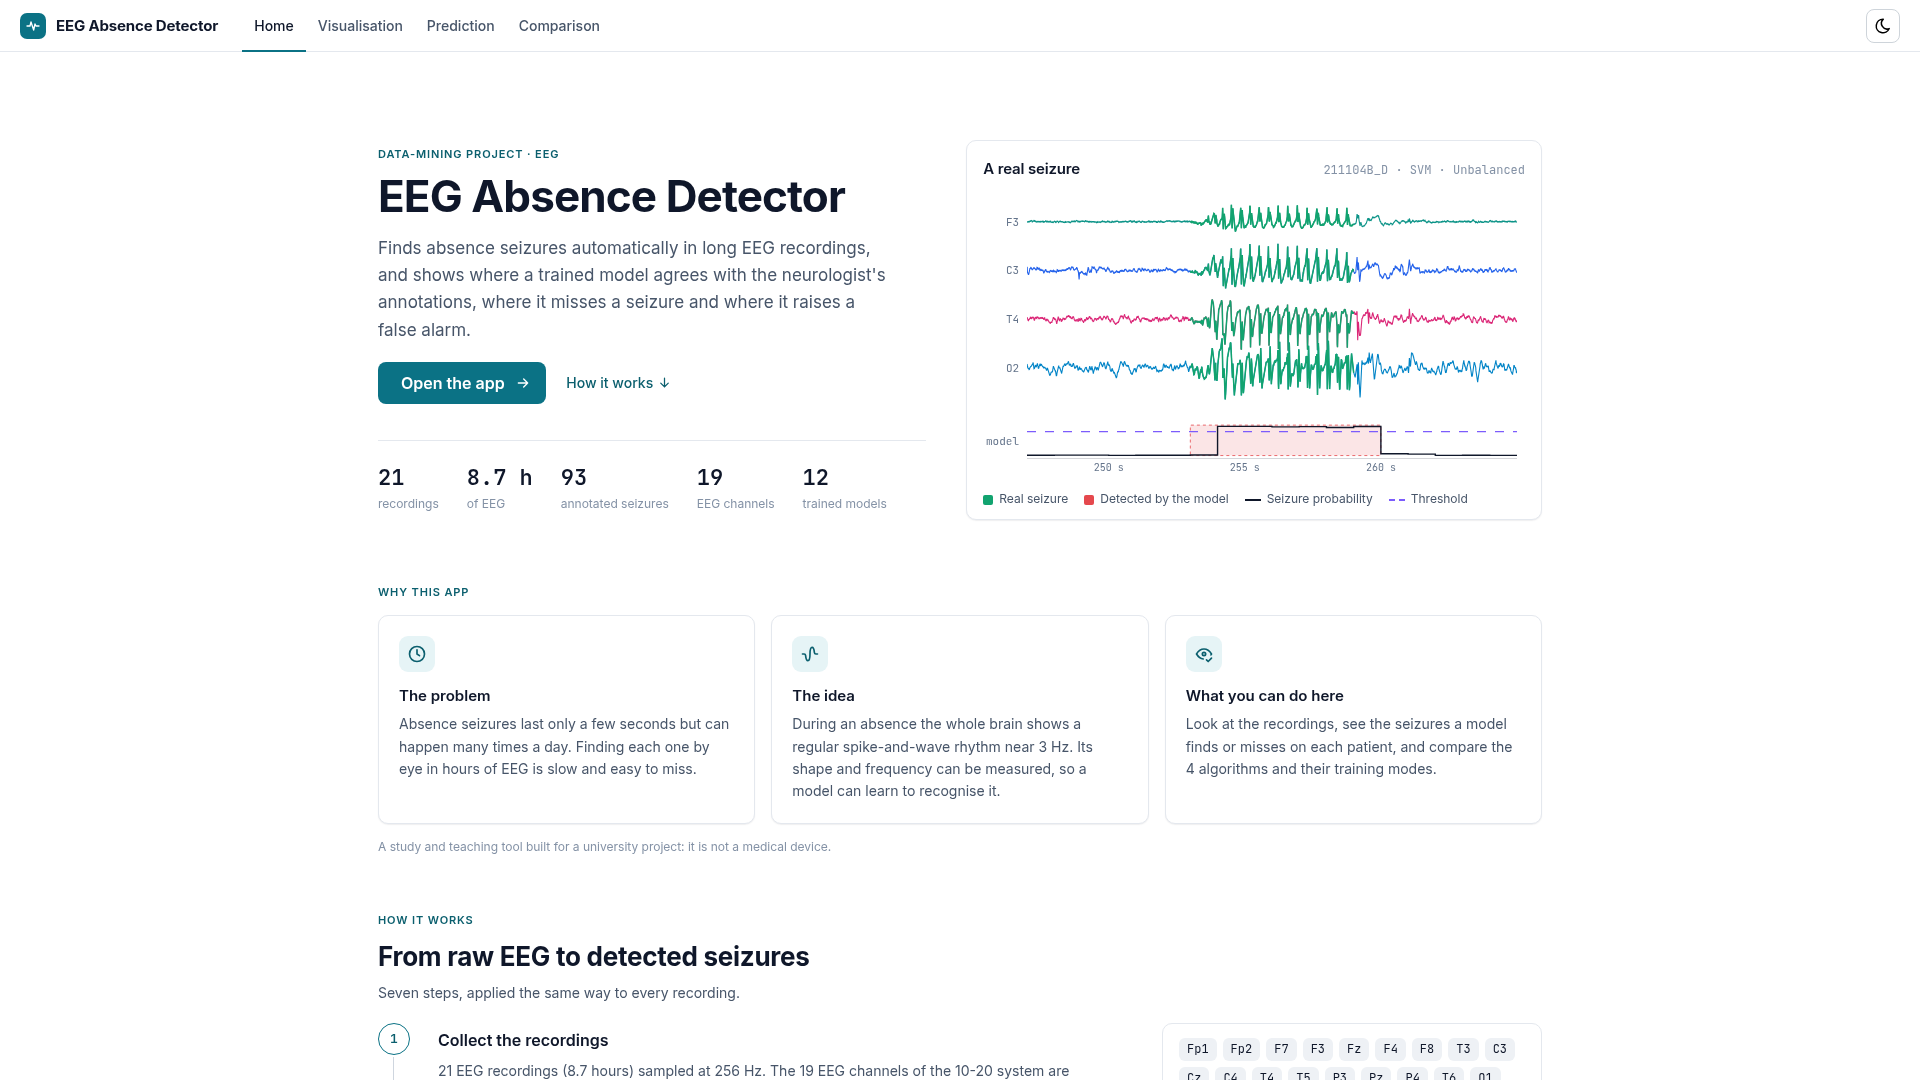
\includegraphics[width=\linewidth]{app/home_light_1920.png}
    \caption{Home}
  \end{subfigure}
  \hfill
  \begin{subfigure}[b]{0.48\linewidth}
    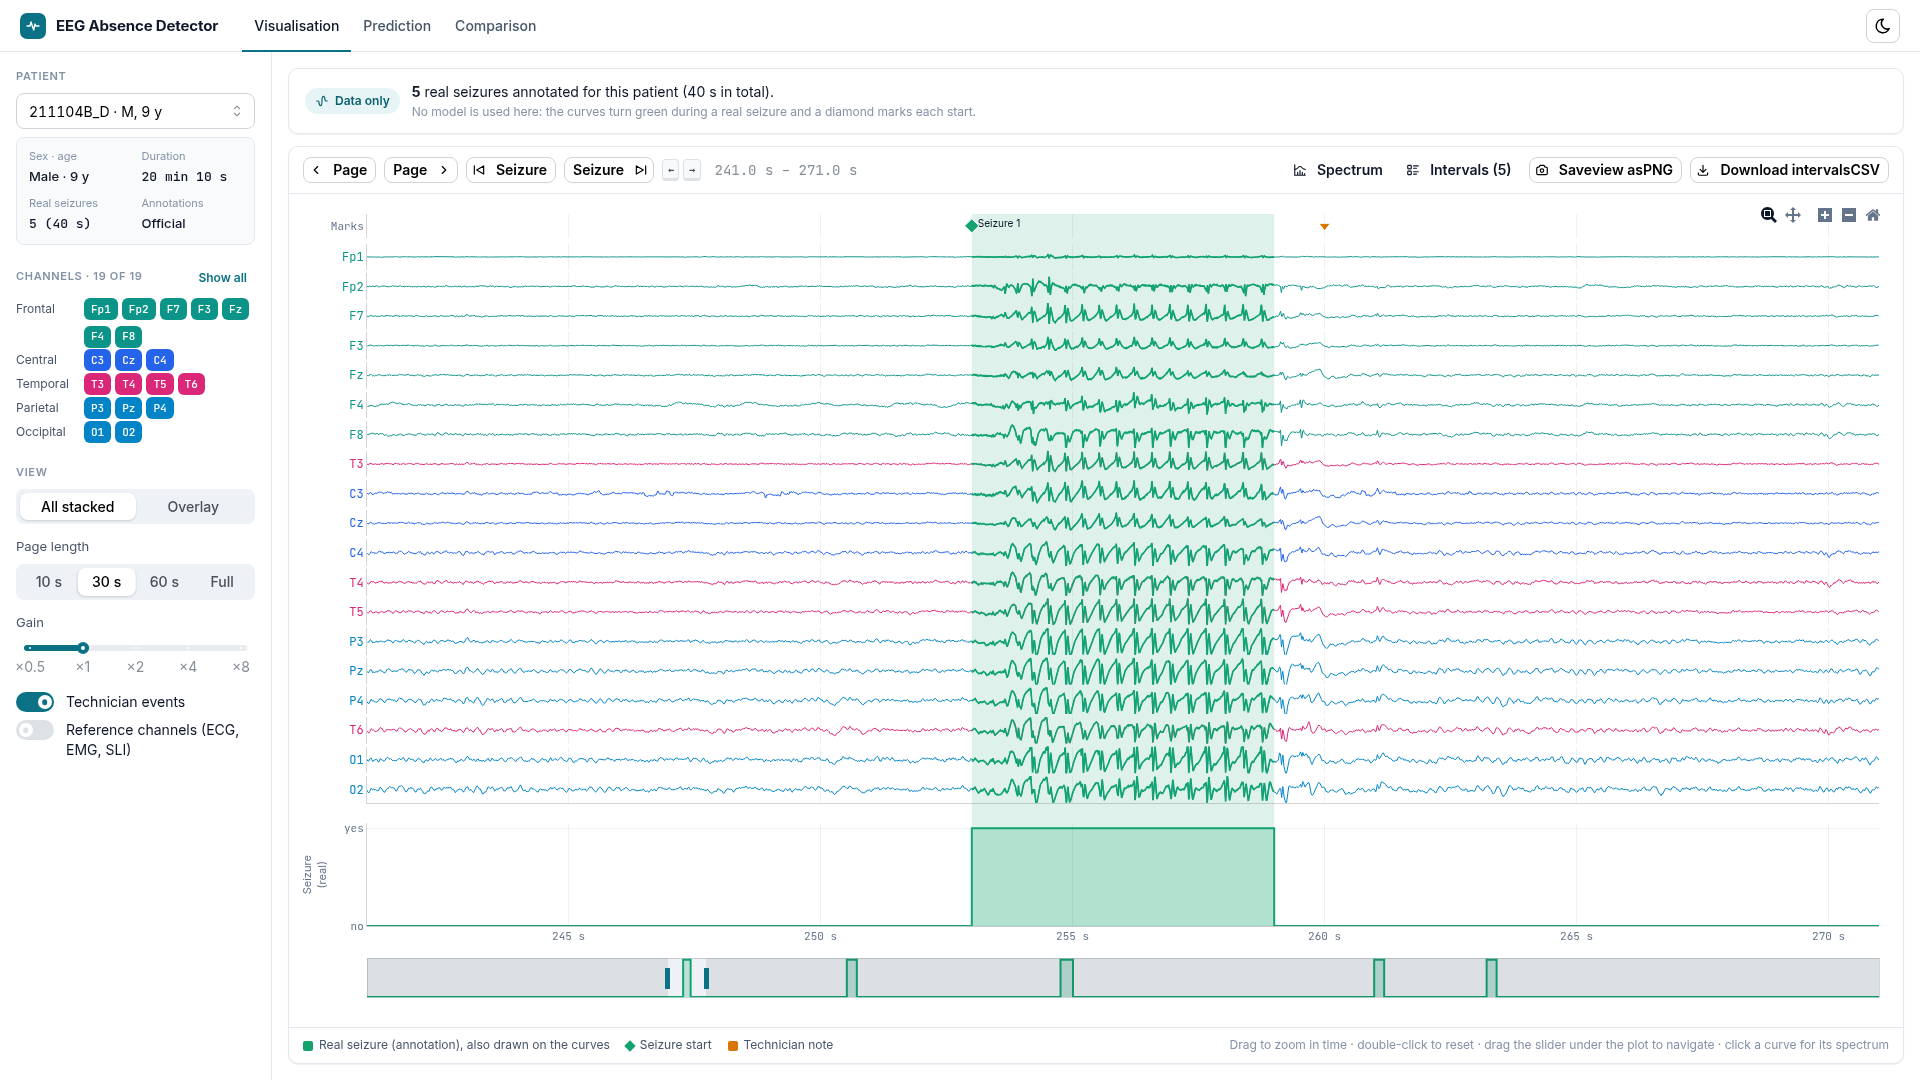
\includegraphics[width=\linewidth]{app/visualisation_light_1920.png}
    \caption{Visualisation}
  \end{subfigure}
  \caption{The Home and Visualisation pages, light theme.}
  \label{fig:app-home-vis}
\end{figure}

\section{Inspecting one patient closely}

The Prediction page is where a single detection can be examined in detail: pick a patient, pick
a model, pick a threshold, and the app shows exactly where that model's probability crosses the
line, against the real annotated seizure and the raw signal underneath it.

\begin{figure}[H]
  \centering
  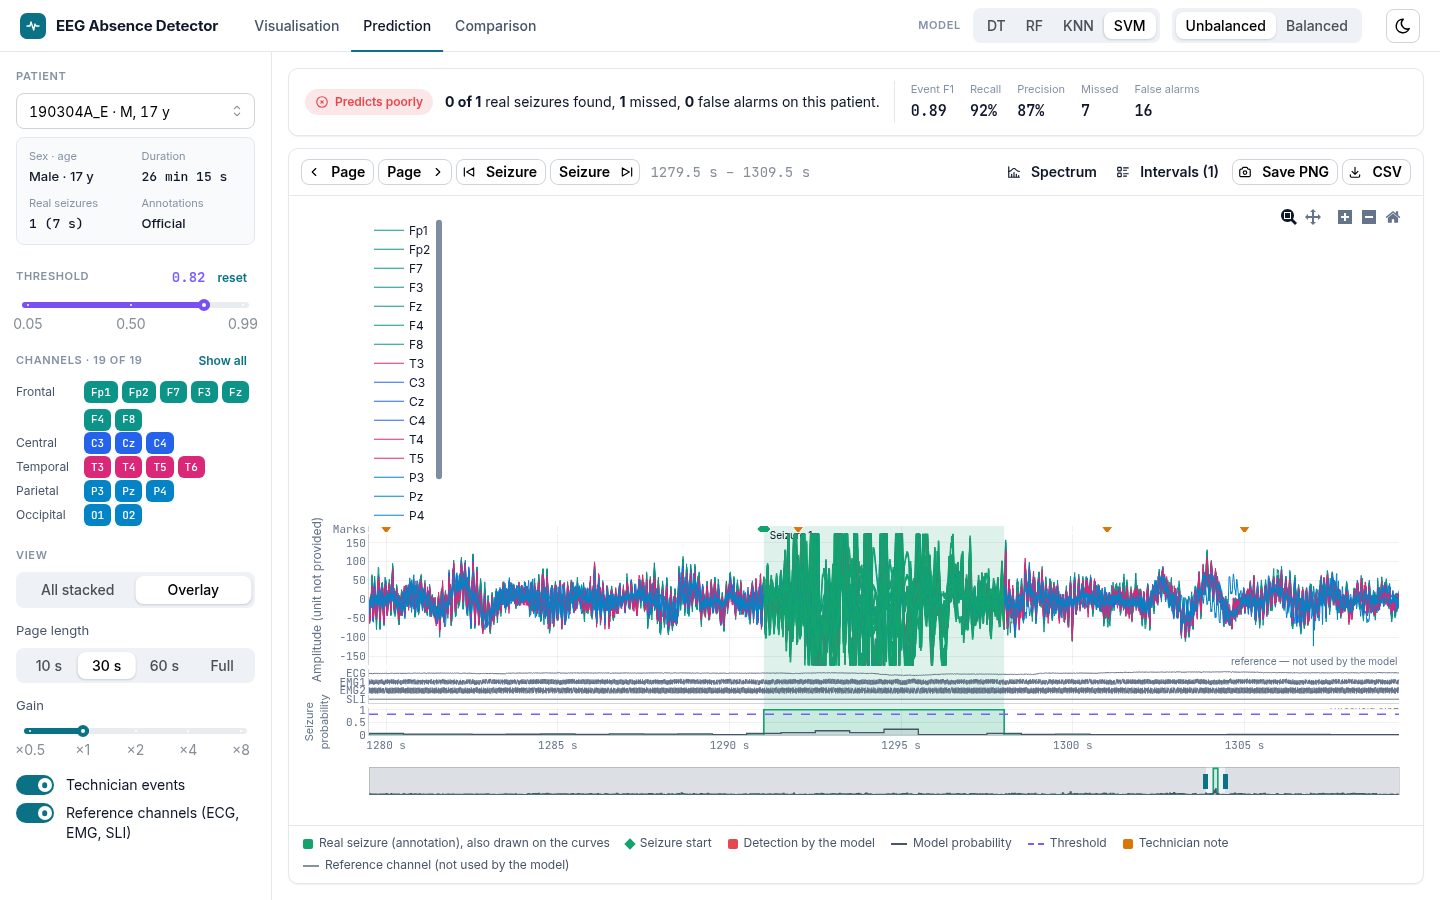
\includegraphics[width=0.92\linewidth]{app/state_overlay_1440.png}
  \caption{Patient \texttt{190304A\_E} on the Prediction page, overlay view: all 19 channels
    drawn on top of one another, with the seizure probability curve and threshold line
    underneath. This is a patient the SVM gets wrong --- the banner reads ``predicts poorly, 0
    of 1 real seizures found'' --- even though the model's numbers across all 21 recordings
    (\Cref{chap:classicalml}) are strong. The real seizure is highlighted in green on both the
    signal and the probability track: the model's probability visibly rises during the event but
    never crosses the 0.82 threshold, the same near-miss pattern already seen in
    \Cref{fig:error-examples}.}
  \label{fig:app-prediction-overlay}
\end{figure}

\section{A calm, clinical design}

The application went through a deliberate visual redesign, moving from its first working
version to a lighter, calmer default theme intended to feel appropriate for a clinical tool
rather than a generic data-science dashboard. The light theme uses a soft, slightly cool
background, white panels, dark slate text, and a single teal accent color; a parallel dark theme
follows the same structure. The 19 EEG channels are colored consistently by scalp region across
both themes.

\begin{figure}[H]
  \centering
  \begin{subfigure}[b]{0.48\linewidth}
    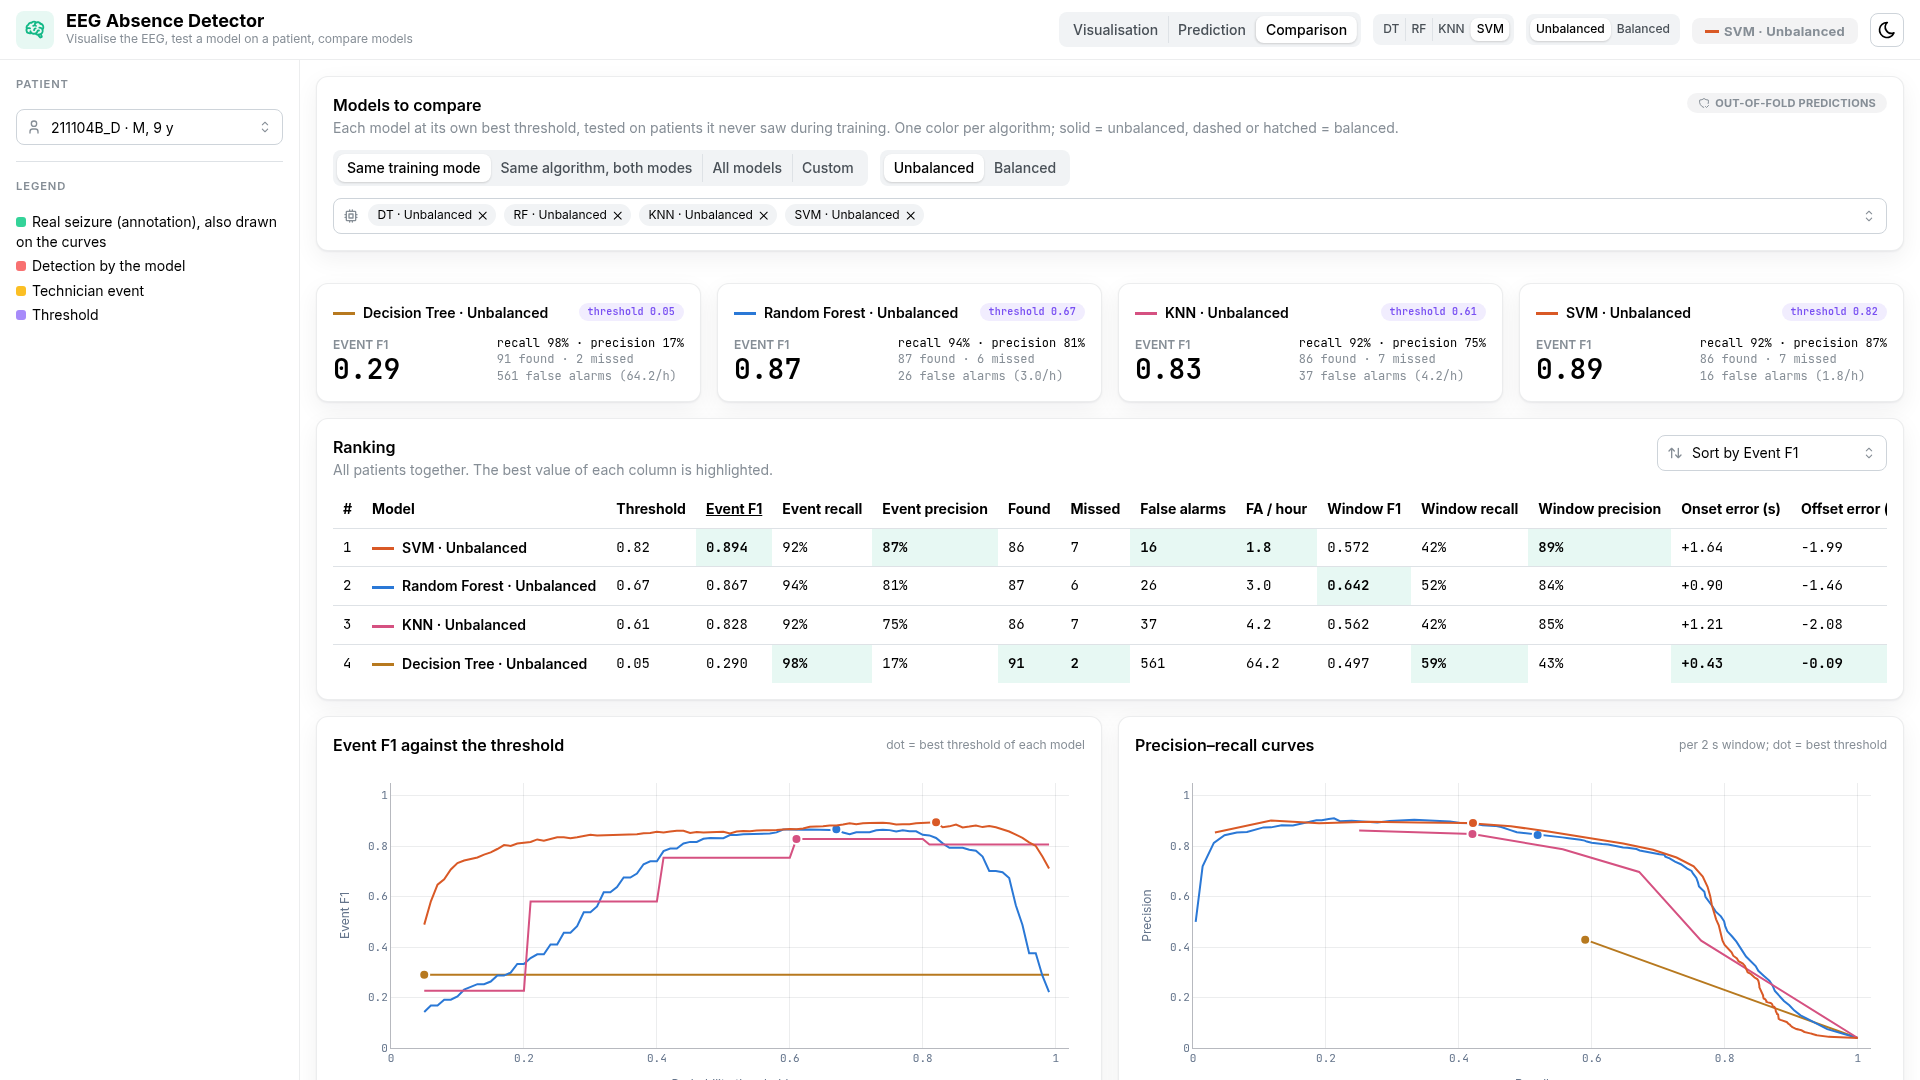
\includegraphics[width=\linewidth]{app/before/comparison_light_1080.png}
    \caption{Before}
  \end{subfigure}
  \hfill
  \begin{subfigure}[b]{0.48\linewidth}
    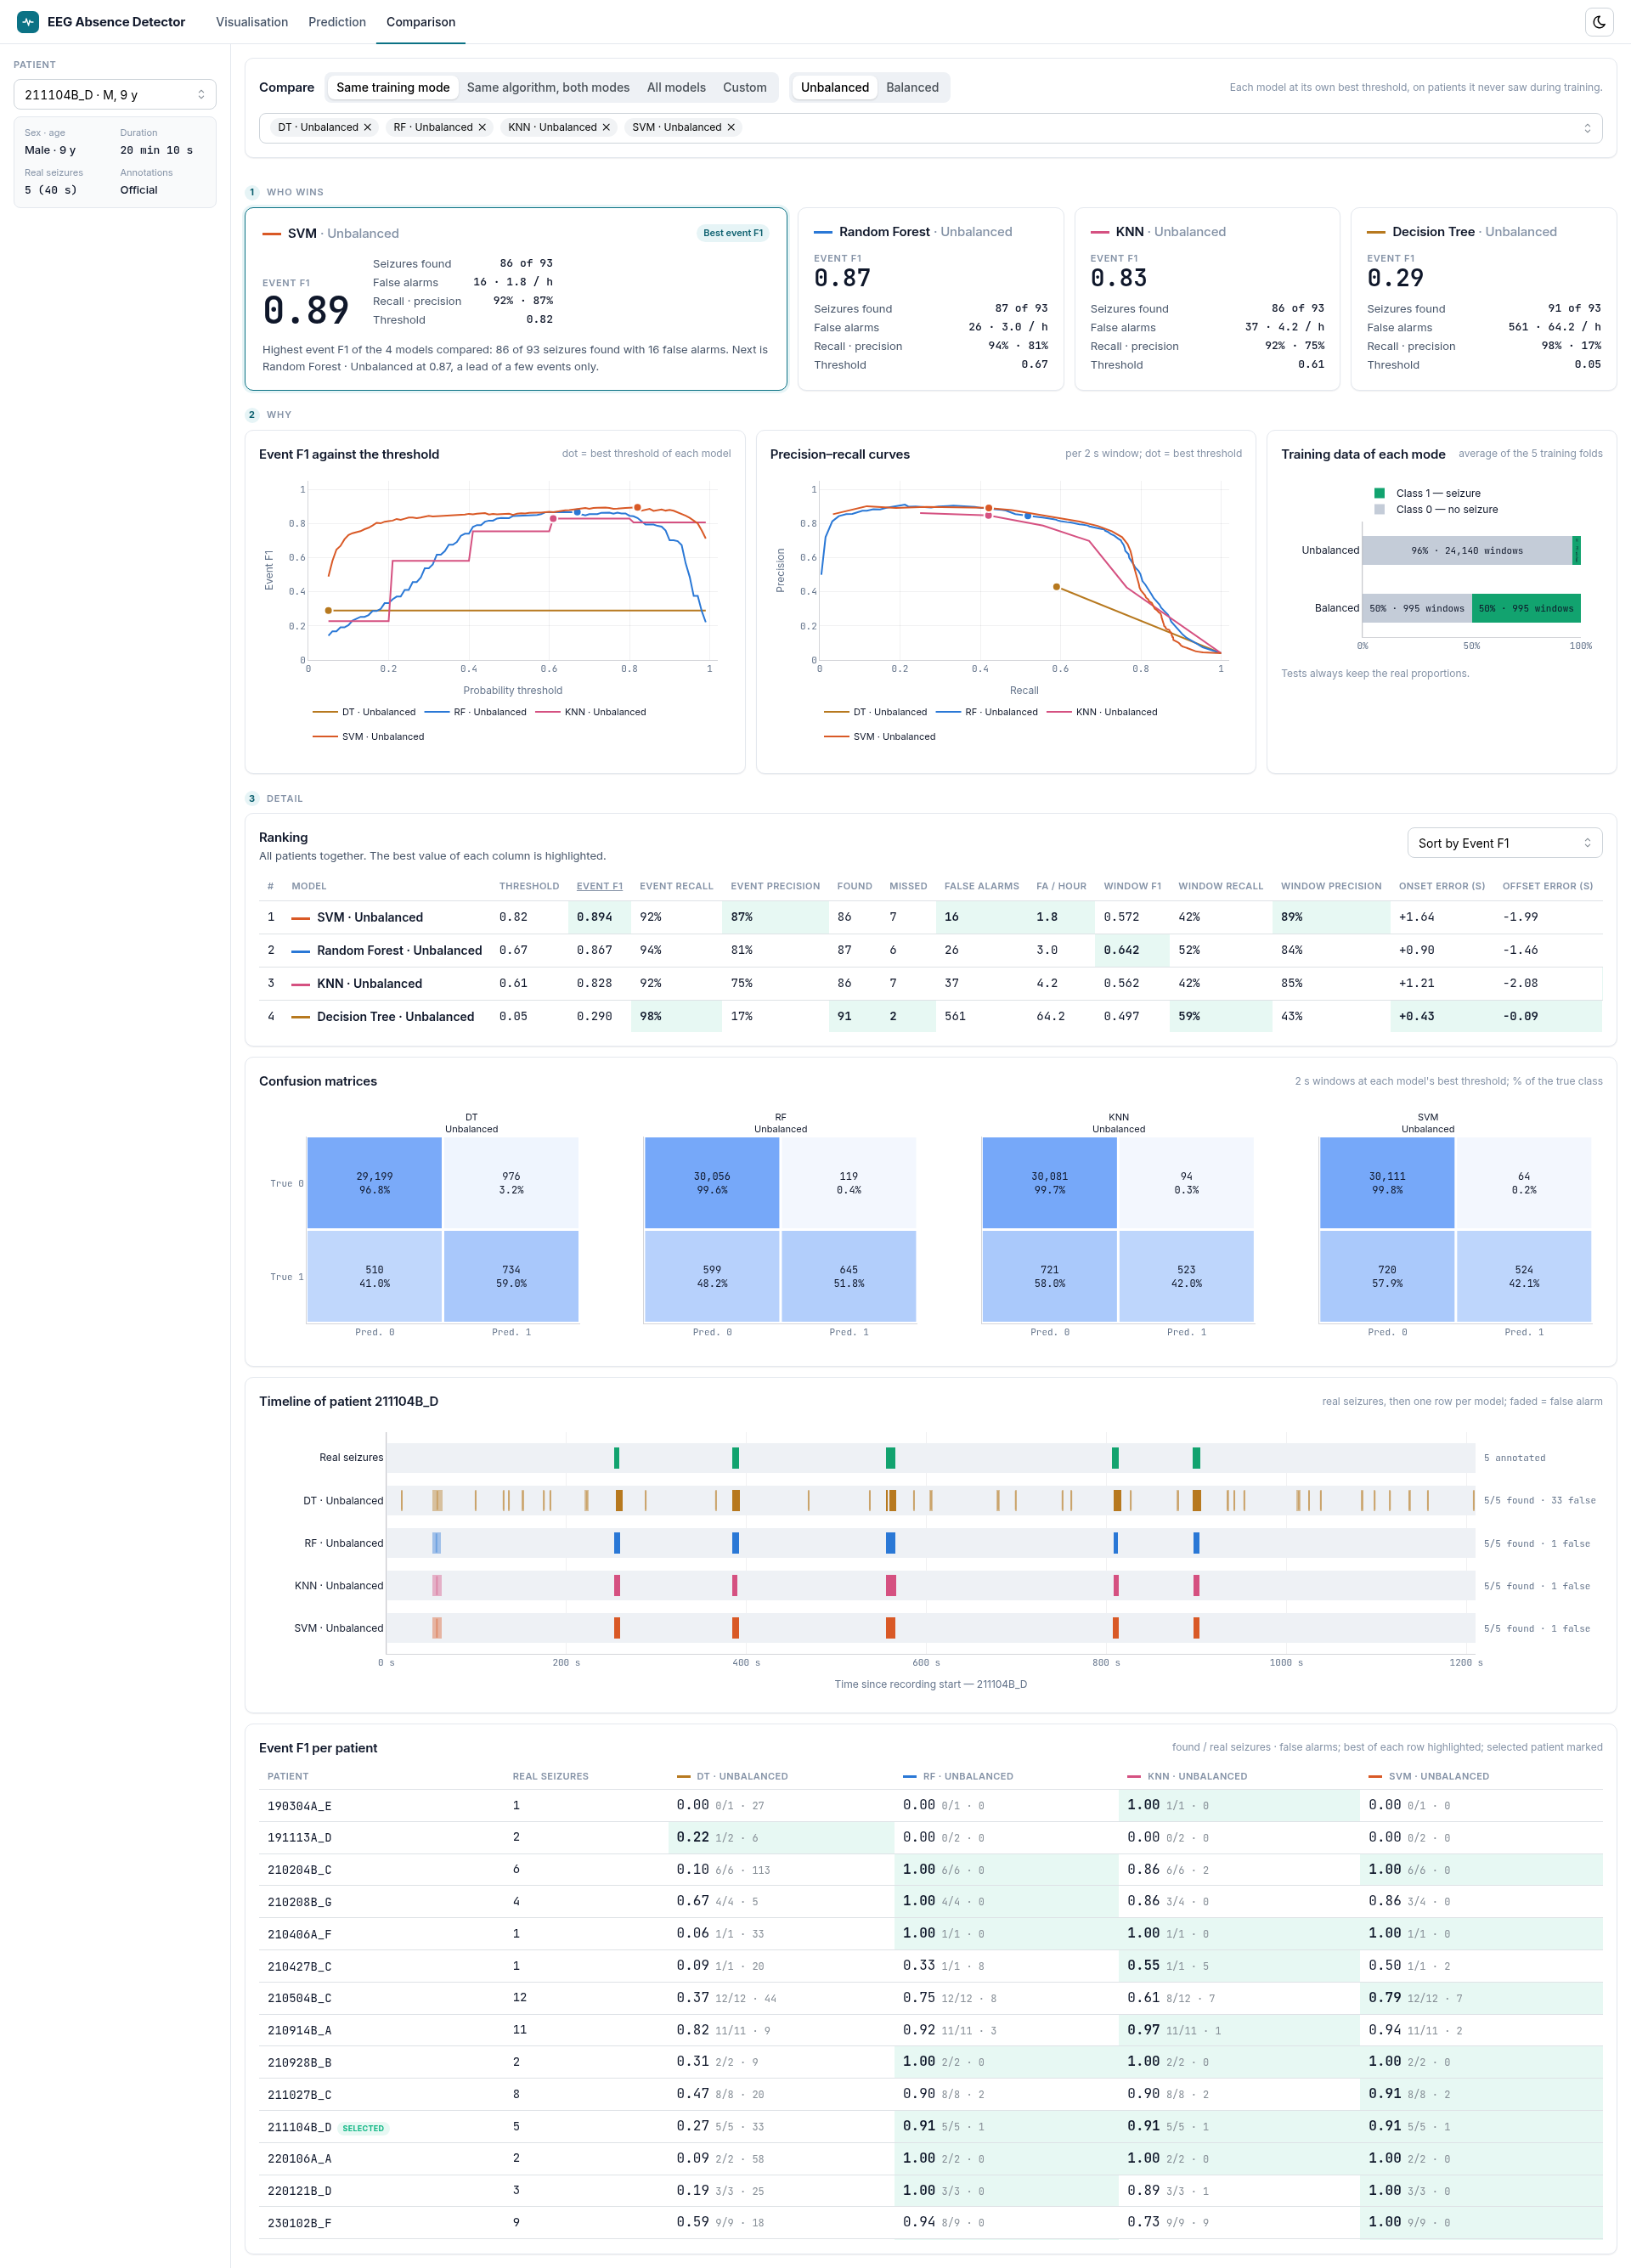
\includegraphics[width=\linewidth]{app/comparison_light_1920.png}
    \caption{After}
  \end{subfigure}
  \caption{The Comparison page before and after the redesign: a denser, plain-gray dashboard
    became a calmer, more explained one, with the same underlying numbers.}
  \label{fig:app-before-after}
\end{figure}

\section{The Comparison page in depth}

The Comparison page's ``all models'' view puts every one of the 12 classical models side by
side for one chosen patient.

\begin{figure}[H]
  \centering
  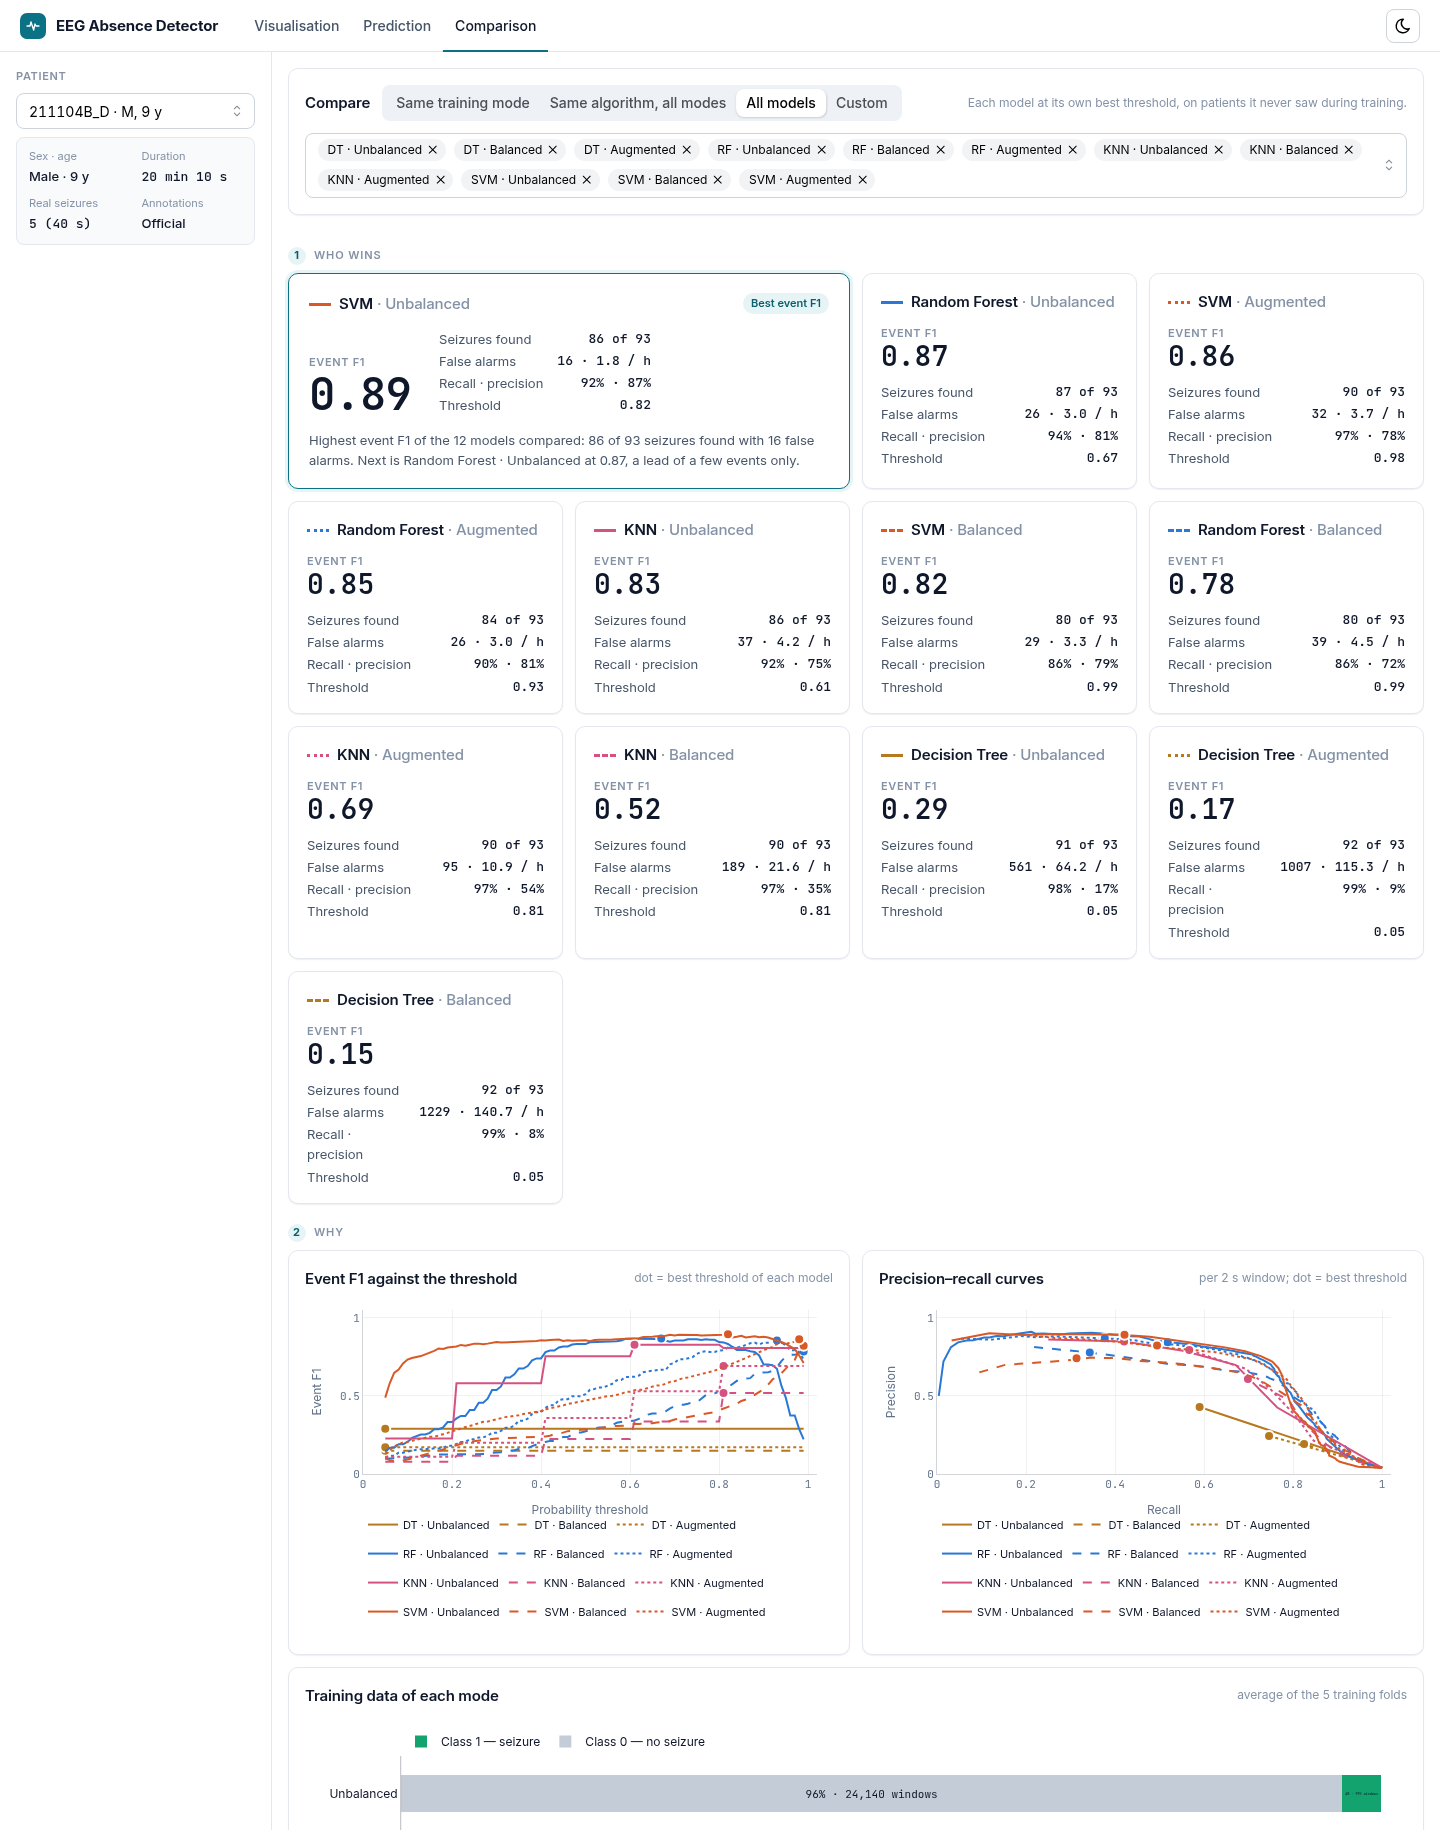
\includegraphics[width=0.92\linewidth]{comparison_depth_a.png}
  \caption{All 12 models selected for patient \texttt{211104B\_D}, each shown as a card with its
    event F1, seizures found, false alarms, recall, precision, and threshold --- SVM unbalanced
    is marked ``Best event F1.'' These numbers (0.89 event F1, 86 of 93 found, 16 false alarms,
    threshold 0.82) match \Cref{tab:classical-results} exactly, since the app reads the same
    underlying results rather than recomputing anything.}
  \label{fig:app-comparison-a}
\end{figure}

\begin{summarybox}
A four-page Dash application --- Home, Visualisation, Prediction, Comparison --- reads only
precomputed results and lets a visitor explore the real EEG signal, a chosen model's detections
down to a single missed seizure on a single patient, and a full 12-model comparison, in a
redesigned, calm clinical visual style. Every number shown in the app traces back to the exact
same results tables used throughout this report.
\end{summarybox}

\chapter{Problems and Lessons Learned}
\label{chap:lessons}

Every project like this accumulates real problems along the way: bad data, bugs, and results
that do not go the way you expected. This chapter collects the ones from this project
honestly, rather than smoothing them out of the narrative.

\begin{enumerate}[leftmargin=1.4em]
  \item \textbf{No absolute clock in the raw files.} The recordings and their annotations each
    started their own internal clock at zero, with no shared reference point anywhere in the raw
    data. Recovering the real offset (\Cref{chap:rawdata}) required rejecting two tempting
    shortcuts that would have quietly fabricated seizure labels.
  \item \textbf{Conflicting annotation rows.} Two recordings had genuinely contradictory seizure
    times in the workbook. Rather than pick a version by hand, each candidate was scored against
    the real EEG signal, and the better-separated candidate was kept --- a repeatable, checkable
    decision instead of a guess.
  \item \textbf{Class imbalance by construction.} Only 3.96\% of windows contain a seizure.
    Balanced training and the first augmentation attempt (shift+mirror) both turned out to
    \emph{hurt} overall event F1 despite improving recall --- a genuine negative result, reported
    in full rather than hidden. The lesson was not to stop there: testing five more augmentation
    methods individually (\Cref{chap:augmentation}) found two, channel dropout and noise, that
    genuinely help, and channel dropout became this project's best result. A negative result for
    the first method tried was not a verdict on the whole approach.
  \item \textbf{A real crash in the CNN training script.} \texttt{event\_counts()} used a pandas
    index label as if it were an array position, which worked by coincidence until a particular
    random validation split exposed it. The bug, how it was found, and the fix are described in
    full in \Cref{chap:deeplearning}.
  \item \textbf{Deep learning did not beat the classical baseline.} This was treated as a
    hypothesis to test, not a result to engineer toward. It did not beat the SVM, and that
    outcome is reported as the finding it is, in \Cref{chap:deeplearning}, rather than reframed
    as a near-win.
  \item \textbf{A long evaluation run had to be killed.} The nested-threshold re-evaluation of
    the classical models (\Cref{chap:evaluation}) is memory-heavy and was killed once for lack of
    available RAM during a full attempt; only 3 models have been scored this way so far. This
    remains an open limitation, not something to paper over, and is listed again in
    \Cref{chap:conclusion}.
  \item \textbf{A naming collision silently overwrote good results.} When bringing new CNN runs
    back from the GPU machine, a quick, one-fold smoke test (meant only to check the training
    script still worked after a code change) happened to reuse the exact output names of two
    already-trained, full, five-fold models. Copying the smoke test's files into place overwrote
    the real results with a tiny, partial run until the mismatch was caught --- the overwritten
    run's window count and found-seizure count were obviously too small for a full run, which is
    what gave it away. The fix was mechanical (restore the real files, re-copy only the genuinely
    new runs), but the lesson is not: any script whose output name depends on its flags needs a
    naming scheme where a debug run and a real run can never collide, and every number brought
    back from an external run is worth a sanity check against what a full run should look like
    before it is trusted.
\end{enumerate}

\begin{summarybox}
Nothing in this project went perfectly on the first try. The raw data needed real detective
work before it could be trusted; two of the three attempts to fix class imbalance made results
worse, not better; a real bug crashed the CNN training script on certain random splits; and a
long-running evaluation script had to be killed for memory. All of it is reported here rather
than quietly cleaned up, because a negative result, honestly reported, is still useful
information.
\end{summarybox}

\chapter{Conclusion and Future Work}
\label{chap:conclusion}

\section{What this project achieved}

Starting from 22 raw clinical recordings with no declared sampling rate, no declared amplitude
unit, and seizure annotations that needed real reconciliation against the signal itself, this
project built a complete, working pipeline for detecting absence seizures in EEG: a cleaned
21-recording, 93-seizure dataset; a documented, zero-phase filtering and feature-extraction
pipeline; a wide search across classical models and training strategies, evaluated honestly,
event by event, under a recording-level split; a six-method data-augmentation study with its
real trade-offs reported in full, including the method that produced this project's best result;
a deep-learning comparison covering two architectures and eight augmentation transforms,
including a real bug found and fixed along the way; and a web application that makes every one
of these results explorable, not just readable.

The best result in the whole project is a single model: SVM trained with channel-dropout
augmentation, event F1 0.901, 88 of 93 seizures found, 18 false alarms --- found by testing
several new augmentation methods in isolation rather than accepting the first one tried. No
ensemble of models beats this single model; the best blend only ties it. Deep learning alone,
trained directly on raw signal and swept across 8 different augmentation transforms, does not
beat the feature-engineered classical approach at this dataset size (best CNN: 0.817, a gap of
0.084), which is itself a useful, honestly reported finding: with only 93 seizures across 21
patients, hand-crafted features built with domain knowledge beat a model trying to learn its own
representation from scratch, regardless of how that model is augmented.

\section{Future work}

Several pieces of work are explicitly unfinished, and are listed here rather than implied to be
done:

\begin{itemize}[leftmargin=1.4em]
  \item \textbf{Finish the nested-threshold evaluation.} Only 3 classical models have been
    re-scored under the same nested-threshold protocol used for the CNNs (\Cref{chap:evaluation}),
    and the new best model (SVM, channel dropout) is not one of them. Completing this would make
    the classical-vs-CNN comparison fully fair, removing the small optimism currently present in
    every classical headline number.
  \item \textbf{A clinical review of the false alarms.} Several of the original best model's
    false alarms coincide with hyperpnea or technician notes (\Cref{chap:classicalml}), and some
    may be real, unannotated seizures. A neurologist's review, particularly of recordings
    \texttt{210504B\_C} and \texttt{210427B\_C}, would clarify this and could raise every model's
    measured precision. This review should be repeated for the new best model's own 18 false
    alarms once scheduled.
  \item \textbf{Check whether the channel-dropout gain is real.} The new best SVM's +0.007 F1
    improvement over the original baseline (\Cref{chap:augmentation}) comes from one training
    run. Repeating it with different random seeds would show whether this is a dependable gain
    or a one-off, the same open question the earlier SVM+CNN ensemble result still carries.
  \item \textbf{Verify the CNN deployment path.} An example for loading the trained CNN weights
    exists in the model repository but has never actually been run, since no PyTorch environment
    is available locally.
  \item \textbf{Clean up unused data.} A 2~GB folder of labeled Excel exports is not used by any
    current pipeline step and can be safely removed and rebuilt if ever needed again.
\end{itemize}

\begin{summarybox}
This project set out to build a trustworthy absence-seizure detector and to test it honestly
against a deep-learning alternative. It did both: a wide search across classical models,
training strategies, and six augmentation methods produced a documented best result (event F1
0.901, a single SVM with channel-dropout augmentation --- not an ensemble, not a deep model), and
a clear, evidence-backed answer to the deep-learning question --- not yet, not at this dataset
size, not with any of the 8 augmentation transforms tried. What remains is finishing the fair,
nested evaluation of the best model, and getting a clinician's eyes on the false alarms that
might not be false at all.
\end{summarybox}

\appendix
\chapter{Repository Structure and Commands}
\label{chap:appendix}

\section{Repository layout}

\begin{itemize}[leftmargin=1.4em]
  \item \texttt{data/processed/recordings/<set>/}, \texttt{data/processed/datasets/<name>/} ---
    one folder per recording set and per dataset variant. \texttt{src/paths.py} defines every
    path used by the project's scripts.
  \item \texttt{scripts/} --- one script per pipeline step, each independently runnable.
  \item \texttt{models/} --- \texttt{registry.json} plus the 12 classical \texttt{.joblib}
    models; \texttt{models/cnn/} holds the CNN weights (model classes live in
    \texttt{scripts/train\_cnn.py}, kept self-contained so it can be copied to a GPU machine).
  \item \texttt{app.py} + \texttt{src/app\_*.py} --- the Dash application.
  \item \texttt{docs/} --- one Markdown report per topic.
\end{itemize}

\section{Key commands}

\begin{verbatim}
python app.py
    # run the application

python scripts/build_dataset.py --annotations official
    # rebuild the official 21-recording dataset

python scripts/train_registry.py
    # train the 12 classical models

python scripts/export_cnn_data.py
    # package data for GPU training -> data/cnn/ (never committed)

python scripts/evaluate_cnn.py
    # score the CNNs (reads models/cnn/ and outputs/predictions/)

python scripts/ensemble_predictions.py --models <key> <key>
    # blend already-trained models, no retraining
\end{verbatim}

\section{Dependencies}

Pinned versions, from \texttt{requirements.txt}:

\begin{multicols}{3}
\small
\begin{itemize}[leftmargin=1.2em,itemsep=0pt]
  \item numpy 2.5.3
  \item scipy 1.18.1
  \item pandas 3.0.6
  \item pyarrow 25.0.1
  \item scikit-learn 1.9.1
  \item joblib 1.6.0
  \item mat-io 1.0.0
  \item h5py 3.16.0
  \item openpyxl 3.1.5
  \item XlsxWriter 3.2.9
  \item PyYAML 6.0.3
  \item matplotlib 3.11.2
  \item seaborn 0.13.2
  \item timescoring 0.0.7
  \item dash 4.4.1
  \item dash-mantine-components 2.8.0
  \item dash-iconify 0.1.2
  \item plotly 6.9.0
  \item plotly-resampler 0.11.1
  \item selenium 4.50.0 (optional)
\end{itemize}
\end{multicols}

No PyTorch is listed: CNN training takes place on separate GPU hardware, and only the resulting
weights and predictions are brought back into this repository.


\end{document}
